\documentclass[12pt]{article}

\usepackage{graphicx}
\graphicspath{{figs/}}

\newcommand{\lapl}{\nabla^{2}}
\newcommand{\lr}[1]{\left(#1\right)}
\newcommand{\wh}[1]{\widehat{#1}}
\newcommand{\ua}{\overline{u}}

\usepackage{amsmath, amsfonts}
\usepackage[margin=0.75in]{geometry}
%\usepackage{graphicx}
%\usepackage[pdftex]{graphicx}
\usepackage[dvipsnames]{xcolor}
\newcommand\myshade{85}
\colorlet{mylinkcolor}{violet}
\colorlet{mycitecolor}{YellowOrange}
\colorlet{myurlcolor}{Aquamarine}
\usepackage{hyperref}
\hypersetup{
    pdfstartview={FitH},    % fits the width of the page to the window
    colorlinks=true,       % false: boxed links; true: colored links
    filecolor=magenta,      % color of file links
    linkcolor=mylinkcolor!\myshade!black,
    citecolor=mycitecolor!\myshade!black,
    urlcolor=myurlcolor!\myshade!black,
}

\title{2D Rayleigh Benard Convection}
%\author{}

\begin{document}

  \maketitle

  \section{Governing Equations}
    We will solve for the vertical velocity $v\lr{x,y}$, the horizontal velocity $u\lr{x,y} = \ua\lr{y} + u\lr{x,y}$ 
    (decomposed into the horizontal mean $\ua\lr{y}$ and the fluctuations about the mean $u\lr{x,y}$.  We will 
    also ultimately solve for the temperature field $T\lr{x,y}$ which is the sum of the conduction solution and 
    the departure from the conduction solution (see below).  The nondimensional equations are 
    \begin{align}
      \frac{\partial \lapl v}{\partial t} + \partial_{x}\lr{u\lapl v - v\lapl u} = \nu_{0}\lapl\lapl v \\
      \frac{\partial T}{\partial t} + \mathbf{u}\cdot\nabla T = \kappa_{0}\lapl T \\
      \partial_{x}u + \partial_{y}v = 0 \\
      \frac{\partial \ua}{\partial t} + \partial_{y} \overline{uv} = \nu_{0} {\partial_{y}}^{2}  \ua \label{eq:meanflow}.
    \end{align}
%    \begin{align}
%     \frac{\partial \{u}}{\partial t} = \nu_{0} {\partial_{y}}^{2}  \{u} + \partial_{y} \overline{uv}.
%    \end{align}
    with boundary conditions 
    \begin{align}
      &v = \partial_{y} v = 0, \qquad y = \pm 1 \\
      &u\lr{\pm 1} = 0, \quad T\lr{\pm 1} = \mp 1.
    \end{align}
    We will solve for the temperature departure from the conduction state.  In dimensionless units 
    the conduction solution is $T_{c} = -y$.  The departure from the conduction state is 
    $\theta = T + y$.  The equation and boundary conditions governing $\theta$ are 
    \begin{align}
      \frac{\partial \theta}{\partial t} + &\mathbf{u}\cdot\nabla\theta - v = \kappa_{0}\lapl\theta \\
      &\theta\lr{\pm 1} = 0.
    \end{align}
    We shall use $\mathcal{N}$ to denote the nonlinear terms in the temperature equation.

  \section{Spatial Discretization}
  We use a Fourier basis in the $x$-direction and a Chebyshev basis in the $y$-direction.

  \subsection{$x$-Discretization}
    Taking the Fourier transform in the $x$-direction of the temperature equation gives 
    \begin{align}
      \partial_{t}\wh{\theta}_{l} + \wh{\mathcal{N}}_{l} - \wh{v}_{l} = 
        \kappa_{0}\lr{-\lr{\alpha k_{x}}^{2}\wh{\theta}_{l} + \partial_{y}^{2}\wh{\theta}_{l}}
      \label{eq:Tl}
    \end{align}
    where $\alpha k_{x}$ is the wavenumber.

    The continuity equation becomes,
    \begin{align}
      i\lr{\alpha k_{x}}\wh{u}_{l} + \partial_{y}\wh{v} = 0 \label{eq:cont_l}.
    \end{align}

    Note that we do not take the Fourier transform of the mean flow equation because it is
    has no horizontal component.

%Similarly, the mean flow equation becomes,
%\begin{align}
%\partial_{t}\wh{u}_{l} = \nu_{0} {\partial_{y}}^{2} \wh{u}_l - \partial_{y}\wh{{uv}}_l \label{eq:meanflow_l}.
%\end{align}
%
%for $k_x = 0$.

  \subsection{$y$-Discretization}
    We use Chebyshev expansions in the $y$-direction following very closely Wally's 
    Chebyshev approach.  We let 
    \begin{align}
      \partial_{y}^{2}\wh{\theta}_{l} = \sum_{m=0}^{N_{C}-1}{\wh{b}_{ml}T_{m}\lr{y}} = \mathbf{T}_{N}\lr{y}\wh{\mathbf{b}}_{l}.
    \end{align}
    Note that $\mathbf{P}_{T}$ is the projection matrix from physical to Chebyshev space.  
    We have $\mathbf{P}_{T}\mathbf{T}_{N} = \mathbf{I}$.  Following Wally's Chebyshev ``integration'' method 
    (using the hybrid approach) we have 
    \begin{align}
      &\partial_{y}\wh{\theta}_{l} = D\boldsymbol{\Psi}\lr{y}\wh{\mathbf{b}}_{l} \\
      &\wh{\theta}_{l} = \boldsymbol{\Psi}_{N}\lr{y}\wh{\mathbf{b}}_{l}.
    \end{align}
    Note that the matrices $\boldsymbol{\Psi}\lr{y}$ have the boundary conditions 
    built in automatically (check their form!).  These are the Galerkin modes in the 
    code.  

    Similarly, for the velocity fields we have 
    \begin{align}
      \partial_{y}^{4}\wh{v}_{l} &= \mathbf{T}_{N}\lr{y}\wh{\mathbf{a}}_{l} \\
      %\partial_{y}^{2}\wh{u}_{l} &= \mathbf{T}_{N}\lr{y}\wh{\mathbf{d}}_{l} \\
      \partial_{y}^{2}\ua        &= \mathbf{T}_{N}\lr{y}\mathbf{c}.
    \end{align}
    
%    \begin{align}
%     \partial_{y}^{2}\{u} &= \mathbf{T}_{N}\lr{y}\wh{\mathbf{c}}.
%    \end{align}
    
    This gives, 
    \begin{align}
      \partial_{y}^{3}\wh{v}_{l} &= D3\mathbf{V}\lr{y}\wh{\mathbf{a}}_{l} \\
      \partial_{y}^{2}\wh{v}_{l} &= D2\mathbf{V}\lr{y}\wh{\mathbf{a}}_{l} \\
      \partial_{y}\wh{v}_{l} &= D\mathbf{V}\lr{y}\wh{\mathbf{a}}_{l} \\
      \wh{v}_{l} &= \mathbf{V}\lr{y}\wh{\mathbf{a}}_{l}
    \end{align}
    and 
    \begin{align}
      \partial_{y}\ua &= D\mathbf{U}\lr{y}\mathbf{c} \\
                  \ua &= \mathbf{U}\lr{y}\mathbf{c}.
    \end{align}
%    and 
%    \begin{align}
%      &\partial_{y}\wh{u}_{l} = D\mathbf{U}\lr{y}\wh{\mathbf{d}}_{l} \\
%      &\wh{u}_{l} = \mathbf{U}\lr{y}\wh{\mathbf{d}}_{l}.
%    \end{align}
    where, once again, the Galerkin modes $\mathbf{V}$ and $\mathbf{U}$ 
    have the appropriate boundary conditions built in.

%    Also,
%    
%    \begin{align}
%    &\partial_{y}\{u} = D\mathbf{U}\lr{y}\wh{\mathbf{c}} \\
%    &\{u} = \mathbf{U}\lr{y}\wh{\mathbf{c}}.
%    \end{align}

    Using the Chebyshev expansions in~\eqref{eq:Tl} gives 
    \begin{align}
      \boldsymbol{\Psi}\lr{y}\partial_{t}\wh{\mathbf{b}}_{l} + \wh{\mathcal{N}}_{l} - 
      \mathbf{V}\lr{y}\wh{\mathbf{a}}_{l} = 
      \kappa_{0}\lr{-\lr{\alpha k_{x}}^{2}\boldsymbol{\Psi}\lr{y}\wh{\mathbf{b}}_{l} + 
                    \mathbf{T}\lr{y}\wh{\mathbf{b}}_{l}}.
    \end{align}
    Finally, we project into Chebyshev space, 
    \begin{align}
      \mathbf{P}_{T}\boldsymbol{\Psi}\lr{y}\partial_{t}\wh{\mathbf{b}}_{l} + \mathbf{P}_{T}\wh{\mathcal{N}}_{l} - 
      \mathbf{P}_{T}\mathbf{V}\lr{y}\wh{\mathbf{a}}_{l} = 
      \kappa_{0}\lr{-\lr{\alpha k_{x}}^{2}\mathbf{P}_{T}\boldsymbol{\Psi}\lr{y} + \mathbf{I}}\wh{\mathbf{b}}_{l}.
    \end{align}

    Note that we will only use the continuity equation to solve for the horizontal velocity 
    perturabation.  Further note that the horizontal velocity perturbation only appears in 
    the nonlinear terms in each equation.  The nonlinear terms are computed in physical space 
    (since we're using a pseudospectral method) and so we never actually need the horizontal 
    velocity perturbation in Chebyshev space.  With this in mind, we proceed to compute the 
    relevant derivatives of the horizontal velocity perturbation that will be used in the 
    nonlinear terms in each of the main evolution equations (temperature, vertical velocity, 
    and mean flow).  We have, 
    \begin{align}
      \partial_{x}u + \partial_{y}v = 0.
    \end{align}
    Taking the Fourier transform gives 
    \begin{align}
      \wh{u}_{l}\lr{y} = \frac{i}{\alpha k_{x}} \partial_{y}\wh{v}_{l}\lr{y}.
    \end{align}
    Expanding the $y$-derivative of $v$ in Chebyshev modes leads to,
    \begin{align}
      \wh{u}_{l}\lr{y} = \frac{i}{\alpha k_{x}} D\mathbf{V}\lr{y}\wh{\mathbf{a}}_{l}.
      \label{eq:uly}
    \end{align}
    We will also need the first derivative in $y$ of the horizontal velocity perturbation.  
    We begin by taking the $y$-derivative of the continuity equation, 
    \begin{align}
      \partial_{x}\partial_{y}u + \partial_{y}^{2}v = 0.
    \end{align}
    After taking the Fourier transform we get, 
    \begin{align}
      \partial_{y}\wh{u}_{l} = \frac{i}{\alpha k_{x}}\partial_{y}^{2}\wh{v}_{l}.
    \end{align}
    Expanding in Chebyshev modes results in 
    \begin{align}
      \partial_{y}\wh{u}_{l}\lr{y} = \frac{i}{\alpha k_{x}}D2\mathbf{V}\lr{y}\wh{\mathbf{a}}_{l}.
      \label{eq:dyuly}
    \end{align}

%    Using the Chebyshev discretization in the continuity equation~\eqref{eq:cont_l} gives 
%    \begin{align}
%      i\lr{\alpha k_{x}}\mathbf{U}\wh{\mathbf{d}}_{l} + D\mathbf{V}\wh{\mathbf{a}}_{l} = 0.
%    \end{align}
%    Projecting into Chebyshev space results in 
%    \begin{align}
%      i\lr{\alpha k_{x}}\mathbf{P}_{T}\mathbf{U}\wh{\mathbf{d}}_{l} + \mathbf{P}_{T}D\mathbf{V}\wh{\mathbf{a}}_{l} = 0.
%    \end{align}
%    When $k_{x} \neq 0 $ we can solve for the horizontal velocity modes $\displaystyle \wh{\mathbf{d}}_{l}$. 
%    When $k_{x} = 0$ we need to write a separate equation for the mean flow.

    The mean flow equation~\eqref{eq:meanflow} using the Chebyshev expansions becomes,
    \begin{align}
      \mathbf{U}\lr{y}\partial_{t}\mathbf{c} + \mathcal{N}_{u} = \nu_{0}\mathbf{T}_N\lr{y}\mathbf{c}
    \end{align} 
    where  $\mathcal{N}_{u} = \partial_{y}\overline{uv}$.
    
    After projection into Chebyshev space, we have,
    \begin{align}
      \mathbf{P}_{T}\mathbf{U}\lr{y}\partial_{t}\mathbf{c} + \mathbf{P}_{T}\mathcal{N}_{u} = 
      \nu_{0}\mathbf{I}\mathbf{c} .
    \end{align}

    Our notation regarding the nonlinear term is a bit strange.  However, we shall discuss
    how this term is computed which will shed some light on our notation of choice.  First, 
    we rewrite the nonlinear term as 
    \begin{align}
      \partial_{y}\overline{uv} = \overline{u\partial_{y}v} + \overline{v\partial_{y}u}.
    \end{align}
    Note that in the code each term is in Fourier space.  Here are some steps for computing the 
    nonlinear term:
    \begin{enumerate}
      \item The first step is to inverse transform from wavenumber space to $x$-space.  
      \item Then, using~\eqref{eq:uly} and~\eqref{eq:dyuly} we can bring each term into physical space.  
      \item Next compute the average in the $x$-direction.  
      \item At this point, we have computed the nonlinear term in physical space.  The last step is to 
            bring it back into Chebyshev space.  Note that it is not necessary to do a Fourier transform 
            because we have averaged the horizontal direction out.
    \end{enumerate}

    %\begin{align}
    %\boldsymbol{\mathbf{U}}\lr{y}\partial_{t}\wh{\mathbf{c}} + \wh{\mathcal{N}}_u = 
    %\mathbf{T}_N\lr{y}\wh{\mathbf{c}} .
    %\end{align} 
    %
    %where  $\wh{\mathcal{N}}_u =   \partial_{y} \overline{uv}$.  This term is evaluated as follows,
    %\begin{align}
    %\overline{uv} =  \mathbf{T}_N\lr{y}\wh{\mathbf{n}} \\
    %\partial_{y} \overline{uv} = \mathbf{T}_N\lr{y}\wh{\mathbf{m}}.
    %\end{align}
    %where $\wh{\mathbf{m}}$ is computed using 'C2Cder' subroutine (Cheb to Cheb differentiation) from Wally's notes.
    %
    %After projection into Chebyshev space, we have,
    %\begin{align}
    %\mathbf{P}_{T}\boldsymbol{\mathbf{U}}\lr{y}\partial_{t}\wh{\mathbf{c}} + \mathbf{I}\wh{m} = 
    %\mathbf{I}\wh{\mathbf{c}} .
    %\end{align}

  \section{Temporal Discretization}

  \section{Verification and Validation (V\&V)}
  In this section we summarize some of the tests that we performed to verify our code.  We 
  primarily focus on code verification at this point rather than validation.  At some point, 
  we would need to do some validation testing as well.

  \subsection{Mean-Flow Implementation}
    We ran a simulation with $\ua\lr{y,t=0} = 0$ and turned off the nonlinear term.  The 
    test here is to ensure that no mean flow develops.  If a mean flow does develop then 
    we have inadvertently introduced a source into the mean flow equation.  When running 
    this test, the mean flow remained zero for all time.

    The next set of tests involved running a simulation with $\ua\lr{y,t=0} = \ua_{0}\lr{y}$ 
    and no nonlinear term.  In this situation, we have an analytical solution and we can 
    compare our analytical solution to the numerical solution.  We also do a convergence 
    study.  First we did a mesh refinement by factors of $2$ in the $y$-direction and 
    then we did a mesh refinement by factors of $2$ in the $x$-direction.  In each case 
    we plotted the $L_{2}$ error as a function of mesh parameter to make sure that we 
    achieved the correct convergence rate.
    
    \section{Post-processing}
    
    \subsection{Energy Spectra}
    
    In order to find the total energy spectra, we first find the conserved energy term by manipulating the governing equations. The fundamental governing equations for this system are shown below.
    
    
    \begin{align}
    \frac{\partial \vec{u}}{\partial t} + \lr{\vec{u} \cdot \nabla \vec{u}} - \nu_*\lr{\lapl \vec{u}} + \nabla P - T\hat k = 0 \\
    \frac{\partial T}{\partial t} + \mathbf{u}\cdot\nabla T - v = \kappa_{*}\lapl T \\
    \end{align}
    
    We take the inner product of the two equations with $\vec{u}$ and $T$ respectively and add the two equations to get the total energy equation given by,
    
    \begin{align}
    \frac{1}{2}\frac{D\lr{|\vec{u}|^2 + |{T}^2|}}{D t} = \nu_*\vec u \cdot \lr{\lapl \vec{u}} - \vec u \cdot \nabla P  +  2(vT) + \nu_* T \lapl T\\
    \end{align}
    
    \subsection{Momentum Boundary Layer}
    
    The thickness of momentum boundary layer is calculated from the vertical profiles of the squares of normal components of stresses summed over all dimensions $(/partial_x u)^2 + (/partial_y v)^2$ which is a measure of the total magnitude of normal stress. The horizontally averaged profile shows a well defined peak close to the bottom plate as shown in fig 25. The $z$ location corresponding to this peak is defined as the momentum boundary layer thickness. This location is considered to be the location with the strongest plume merging and convolution takes place.
    
    
     \section{Results}
     \subsection{Effect of Mean Flow}
     The presence of mean flow is found to be a deterrent to heat transport. Our simulation results show that the mean flow lowers the average $Nu$ in the flow as shown in fig 1 at $Pr = 4, Ra = 1E7$. This could be due to distortions introduced by the mean flow in the coherent structures responsible for heat transport. A profile of the mean flow at given time instant is shown in fig 2.
     
     \begin{figure}[!htb]
     	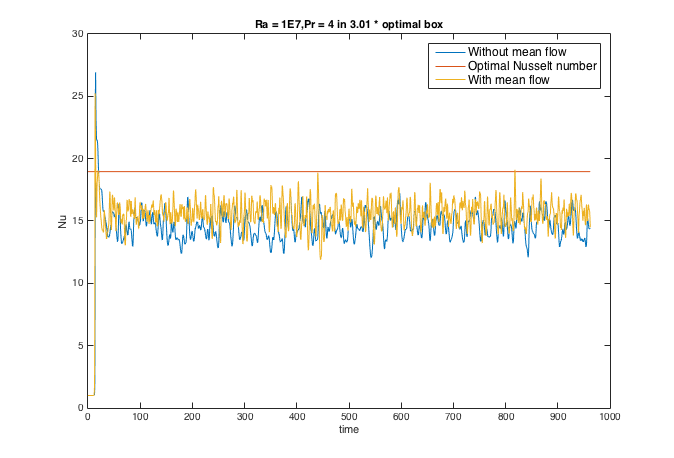
\includegraphics[width=\linewidth]{Nu1E74301opt.png}
     	\caption{Comparison of Nusselt numbers with and without mean flow at $Pr = 4, Ra = 1E7$ in 3.01 X optimal box.}
     	\label{fig:fig1}
     \end{figure}
     
     \begin{figure}[!htb]
     	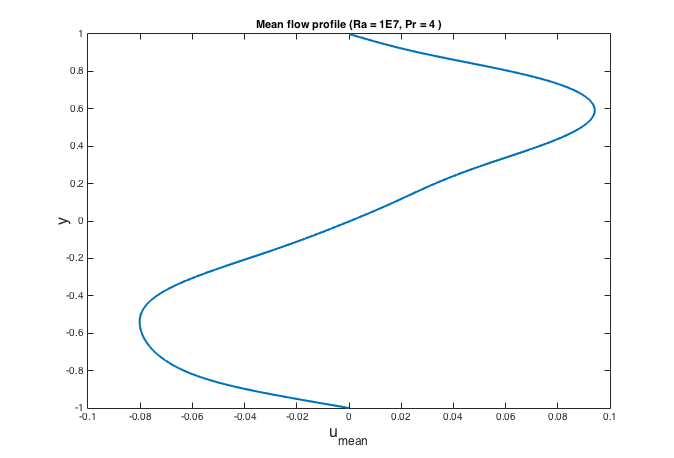
\includegraphics[width=\linewidth]{umean.png}
     	\caption{Mean flow profile at $Pr = 4, Ra = 1E7$ in 3.01*optimal box.}
     	\label{fig:fig1}
     \end{figure}
     
     Therefore, it was decided that the mean flow be omitted in our future studies since it could interfere with the formation of optimal coherent structures whose signatures we are trying to detect.
     
      \subsection{Simulations in the Optimal Box}
      
      Confinement of flow in the optimal box results in the formation of structures very similar to the optimal coherent structures in all the cases that have been looked at so far. In the absence of mean flow, the signature is more pronounced and the averaged structure in a cycle closely resembles the optimal structure as shown fig 3.
      
      \begin{figure}[!htb]
      	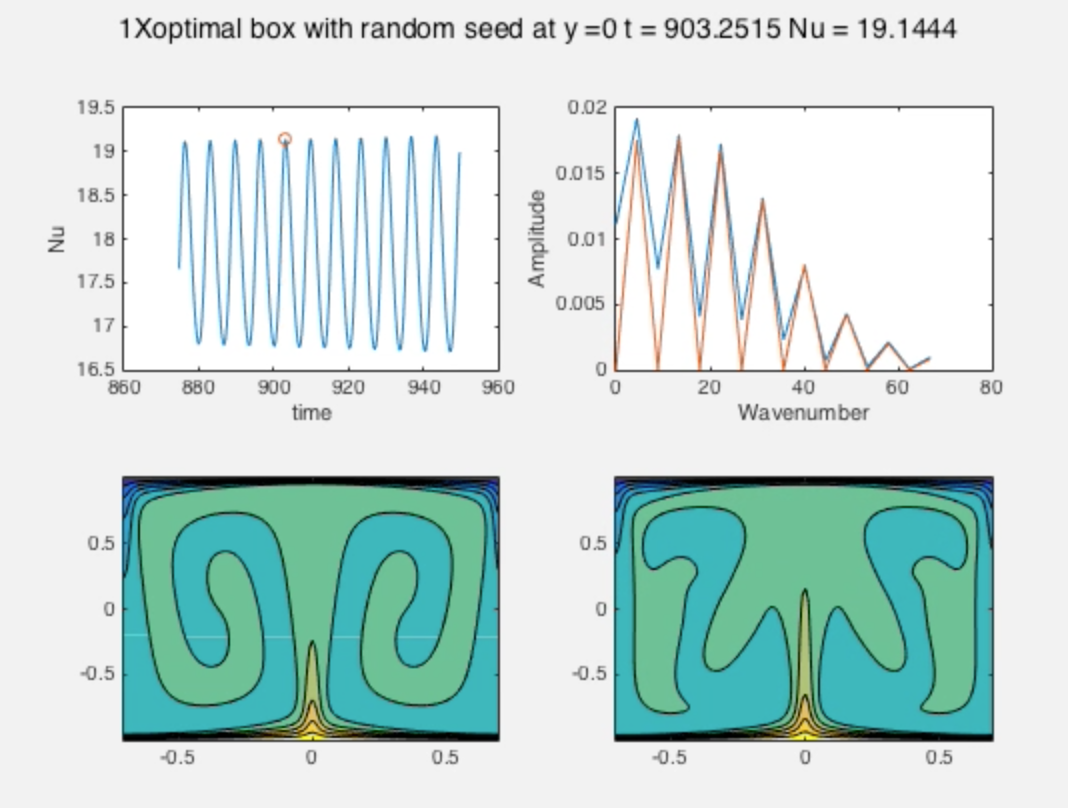
\includegraphics[width=\linewidth]{1E7opt.png}
      	\caption{Flow field at a given time instant, $Pr = 7, Ra = 1E7$ in optimal box}
      	\label{fig:fig3}
      \end{figure}
      
 %     \begin{figure}[!htb]
  %    	\includegraphics[width=\linewidth]{1E7optavg.png}
   %   	\caption{Time-averaged flow field, $Pr = 7, Ra = 1E7$ in optimal box}
    %  	\label{fig:fig3}
     % \end{figure}
      
      The only caveat is that by restricting the flow in the optimal box, turbulence is suppressed; the flow is found to be steady/periodic even at high Rayleigh numbers ($Ra = 1E7$) as shown in fig 4.
      
      \begin{figure}[!htb]
      	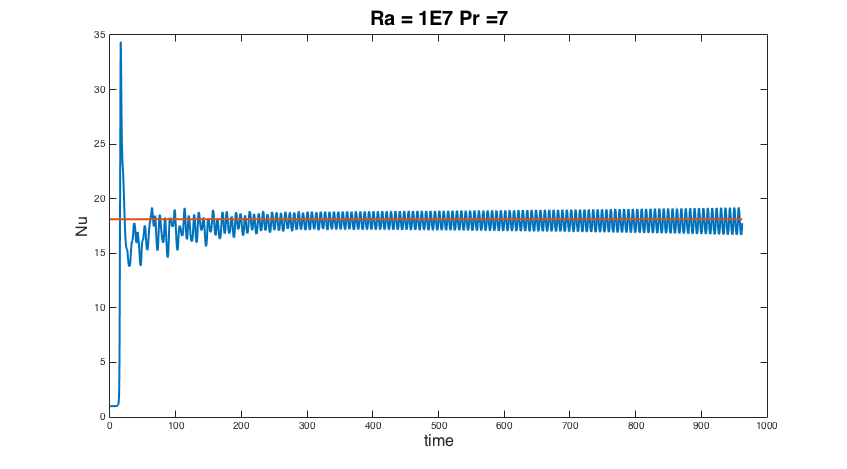
\includegraphics[width=\linewidth]{Nu1E77opt.png}
      	\caption{$Nu$ variation with time at $Pr = 7, Ra = 1E7$ in optimal box (red line denotes the optimal $Nu$).}
      	\label{fig:fig5}
      \end{figure}  
      
      \subsection{Comparison of flow at Ra = 1E7, Pr = 4 in various box sizes}
      
      Simulations were carried out in various boxes where the length is set to be an integral multiple of the optimal box size corresponding to $\alpha_{opt} = alpha = 0.4714574564629509E+001$ at $Ra = 1E7$ and $Pr = 4$. Note that the mean flow is forced to be 0 in all the cases reported.
      
      Figure 6 shows the variation of $Nu$ with time for the different cases and the variation in average $Nu$ with box size is shown in Figure 7. These clearly show that the average Nusselt number keeps dropping with increase in box size. Also note from Figure 6 that the amplitude of oscillations also drops with increase in box size. This may be related to the increased size of the plumes/coherent structures in larger boxes.
      
      \begin{figure}[!htb]
      	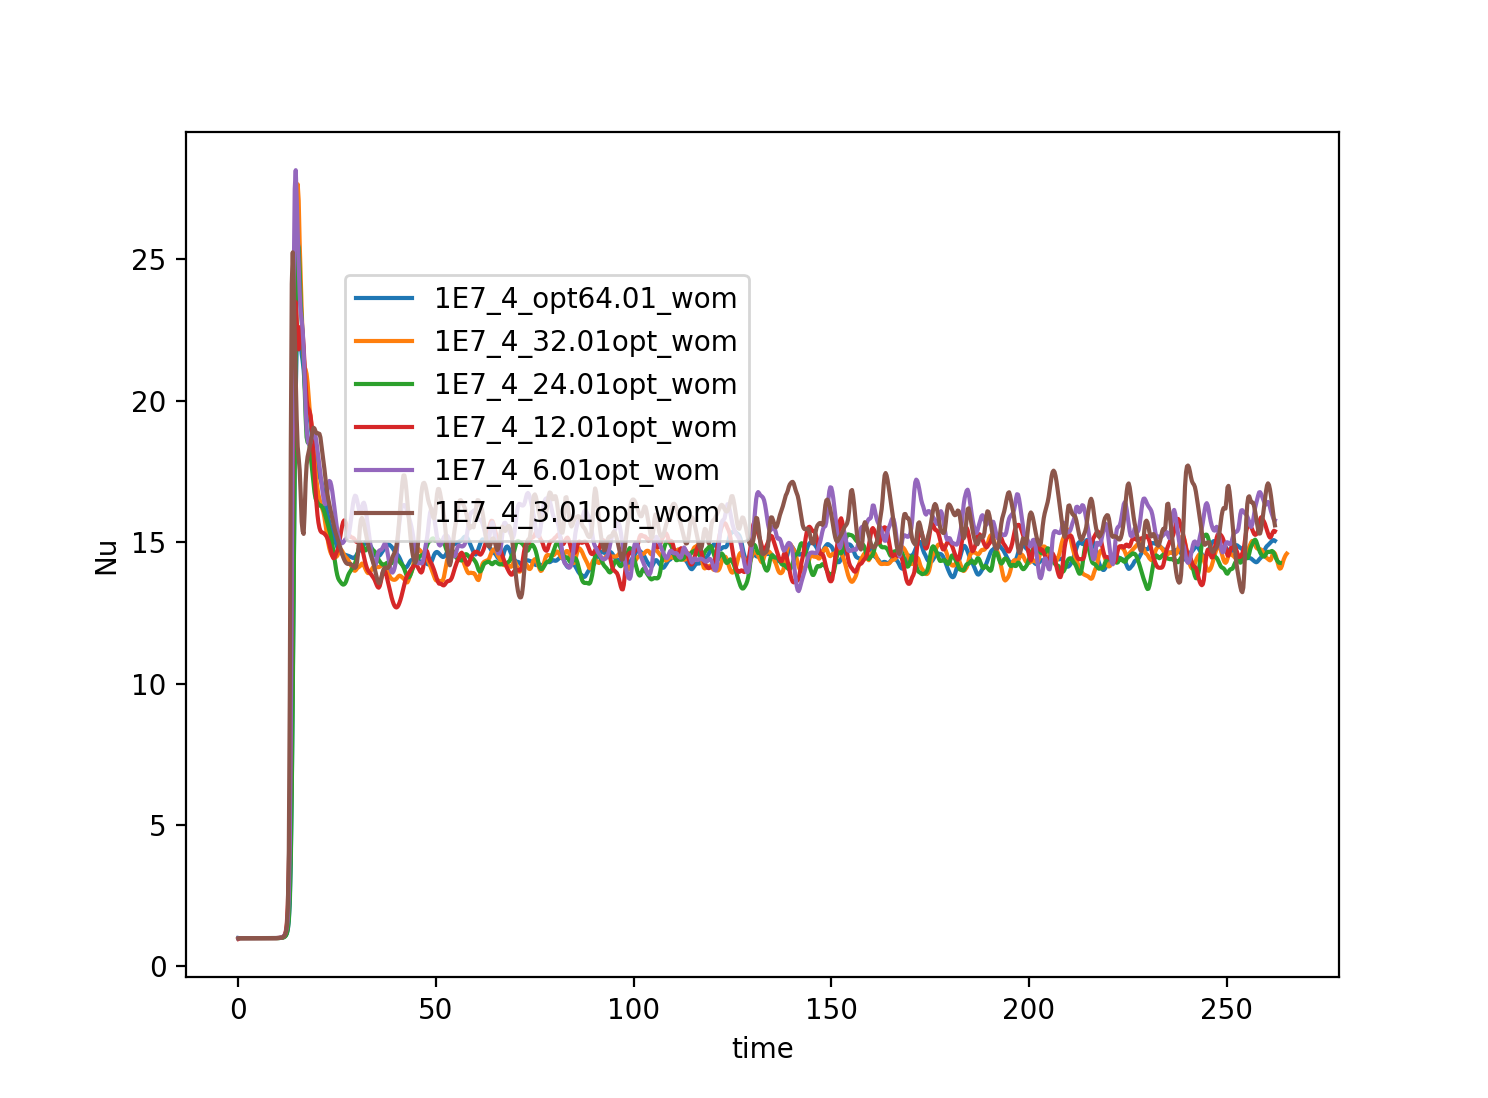
\includegraphics[width=\linewidth]{Nu_1E7_4.png}
      	\caption{$Nu$ variation with time at $Pr = 4, Ra = 1E7$ in various box sizes.}
      	\label{fig:fig6}
      \end{figure} 
      
      \begin{figure}[!htb]
      	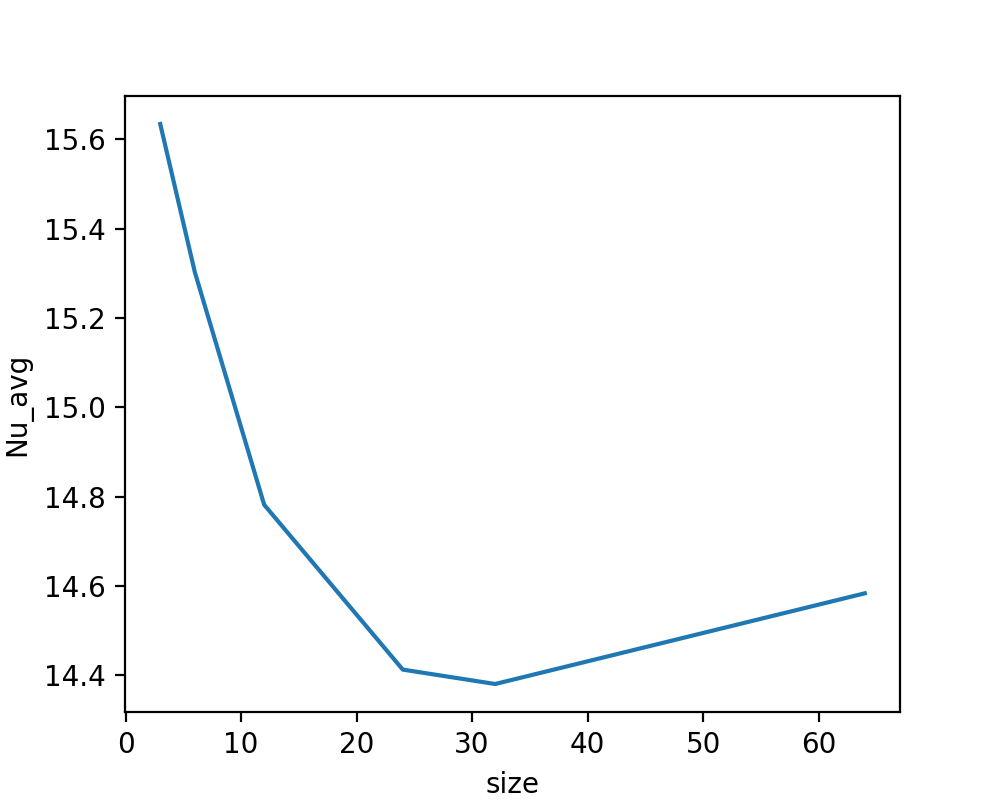
\includegraphics[width=\linewidth]{Nu_avg_1E7_4.png}
      	\caption{$Nu_{avg}$ variation with box size for $Pr = 4, Ra = 1E7$.}
      	\label{fig:fig7}
      \end{figure} 
      
      The contours of $T,u,w$ are plotted in Figures 8-13 for the 5 cases considered. The time is chosen such that the flow has attained a statistically steady state.
      
      \begin{figure}[!htb]
      	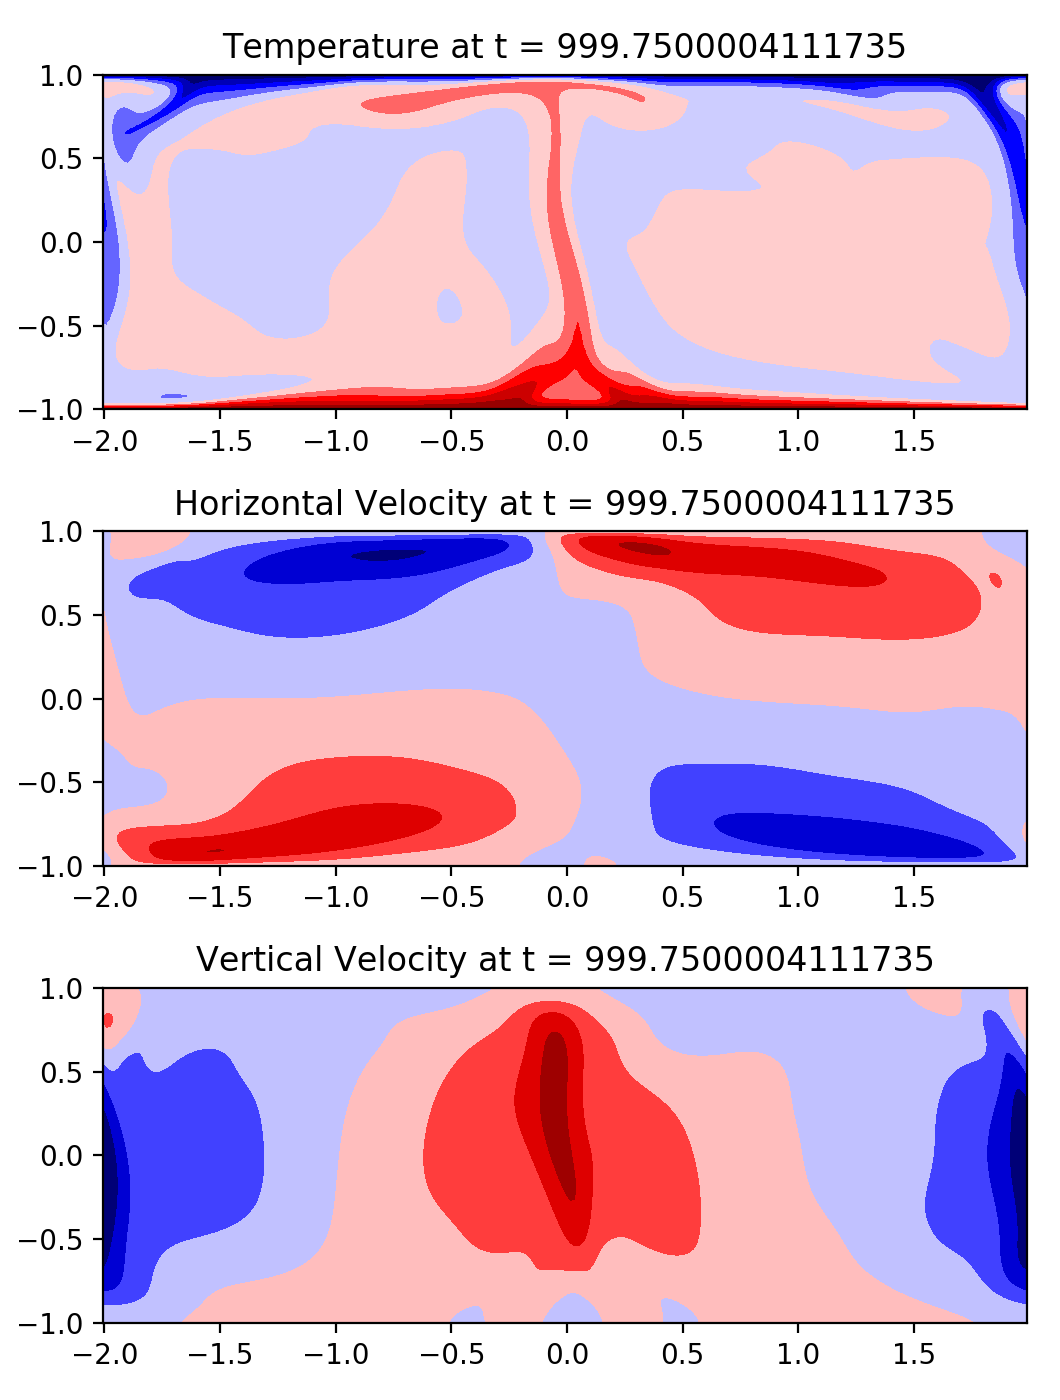
\includegraphics[width=\linewidth]{contours_1E7_4_3.png}
      	\caption{Temperature, horizontal and vertical velocity contours for $Ra = 1E7, Pr =4, l_b = 3* l_{opt} $ }
      	\label{fig:fig8}
      	\end{figure}
      	
      	\begin{figure}[!htb]
      		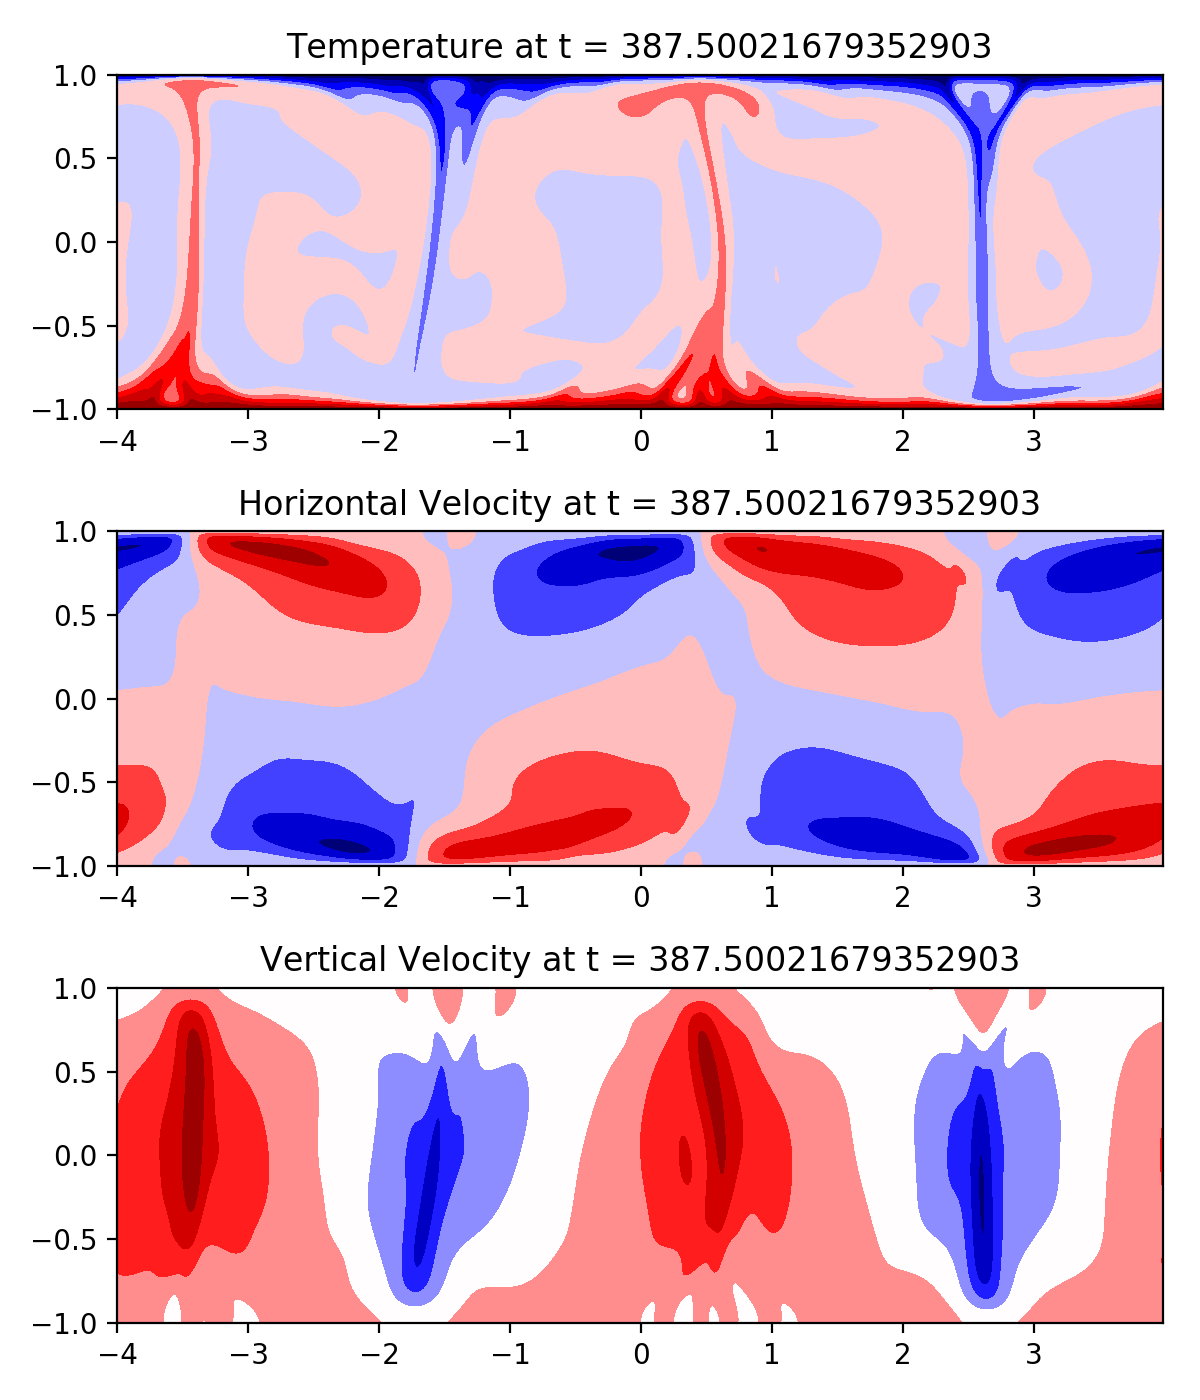
\includegraphics[width=\linewidth]{contours_1E7_4_6.png}
      		\caption{Temperature, horizontal and vertical velocity contours for $Ra = 1E7, Pr =4, l_b = 6* l_{opt} $ }
      		\label{fig:fig9}
      	\end{figure}

   \begin{figure}[!htb]
   	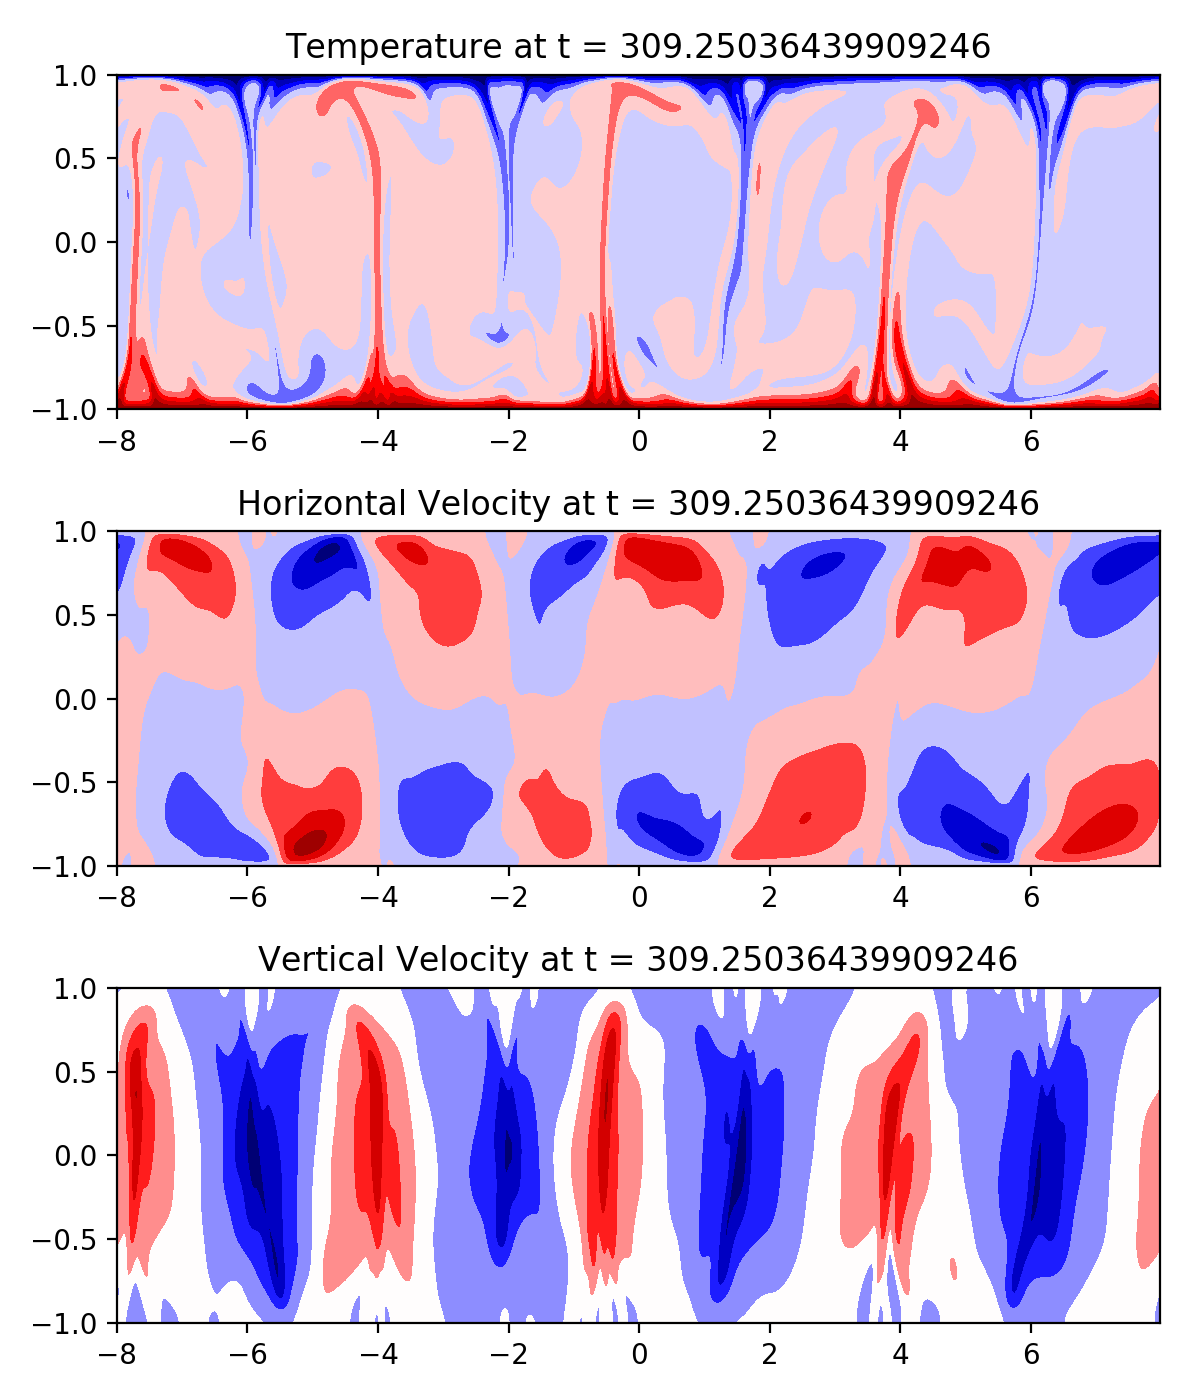
\includegraphics[width=\linewidth]{contours_1E7_4_12.png}
   	\caption{Temperature, horizontal and vertical velocity contours for $Ra = 1E7, Pr =4, l_b = 12* l_{opt} $ }
   	\label{fig:fig10}
   \end{figure}
   
   \begin{figure}[!htb]
   	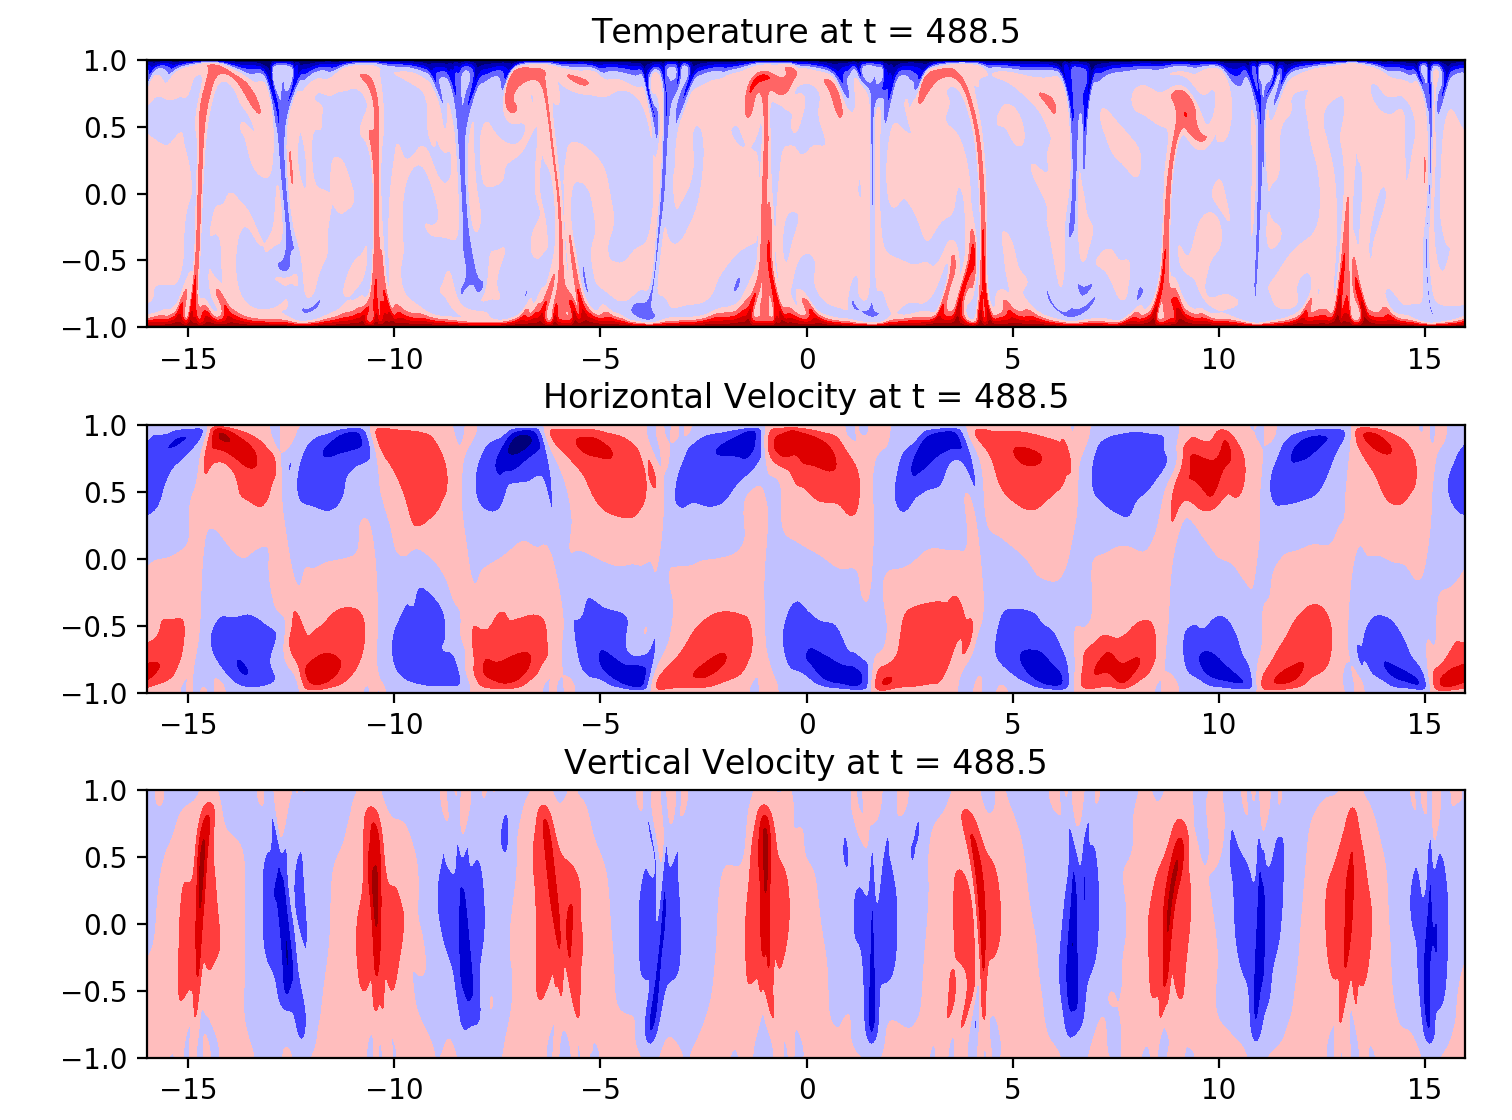
\includegraphics[width=\linewidth]{contours_1E7_4_24.png}
   	\caption{Temperature, horizontal and vertical velocity contours for $Ra = 1E7, Pr =4, l_b = 24* l_{opt} $ }
   	\label{fig:fig11}
   \end{figure}
   
   \begin{figure}[!htb]
   	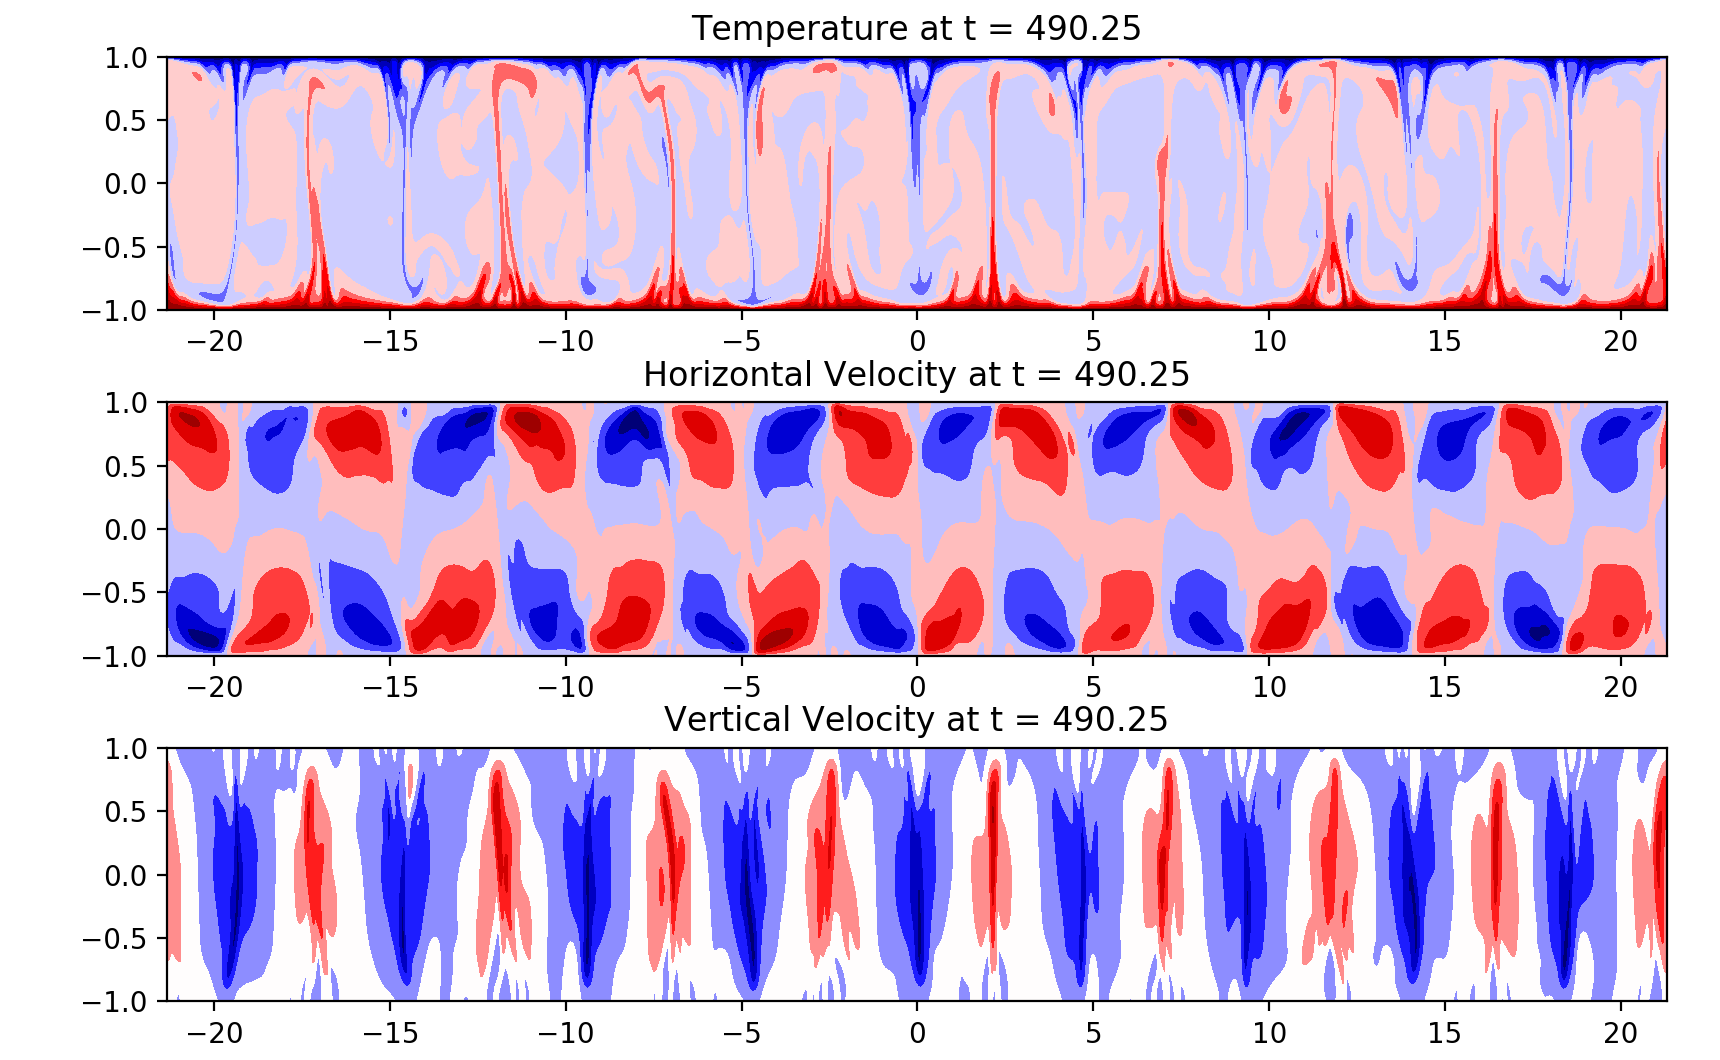
\includegraphics[width=\linewidth]{contours_1E7_4_32.png}
   	\caption{Temperature, horizontal and vertical velocity contours for $Ra = 1E7, Pr =4, l_b = 32* l_{opt} $ }
   	\label{fig:fig12}
   \end{figure}

 \begin{figure}[!htb]
 	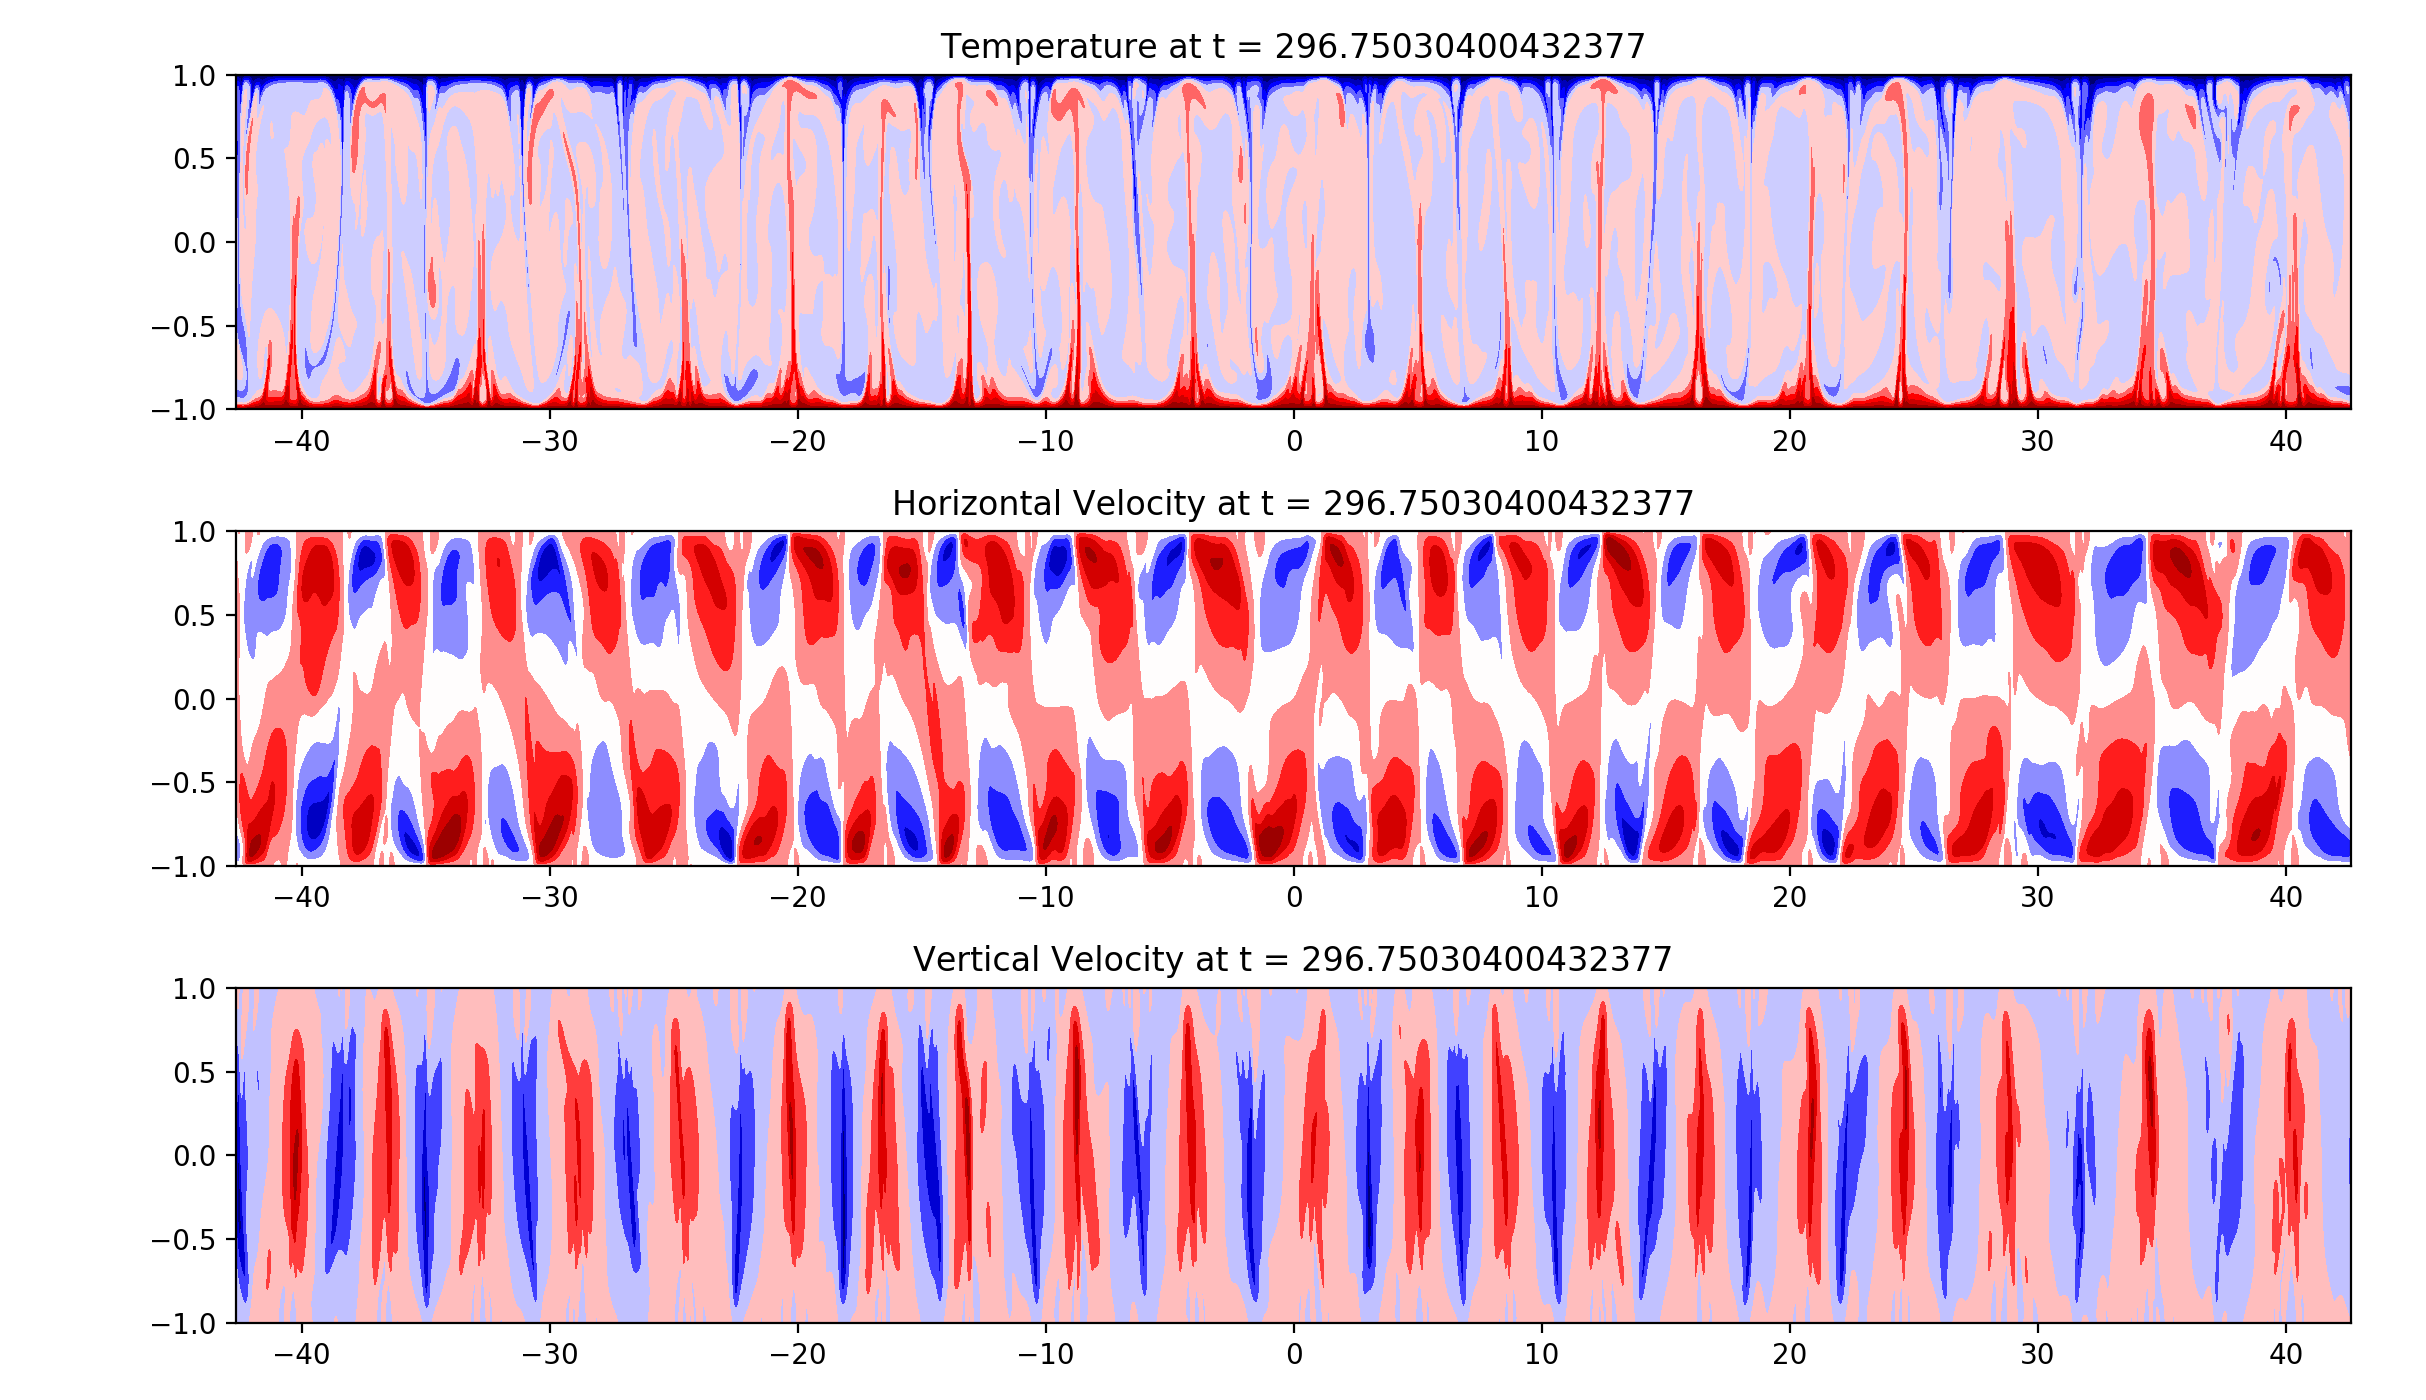
\includegraphics[width=\linewidth]{contours_1E7_4_64.png}
 	\caption{Temperature, horizontal and vertical velocity contours for $Ra = 1E7, Pr =4, l_b = 64* l_{opt} $ }
 	\label{fig:fig12}
 \end{figure}

A comparison of the energy spectra for the various cases are shown in Figures 13-15. The energy spectra is plotted along $y = 0$. Note that the length scale corresponding to the largest energy in all 3 cases keeps decreasing with increase in box size.

  \begin{figure}[!htb]
  	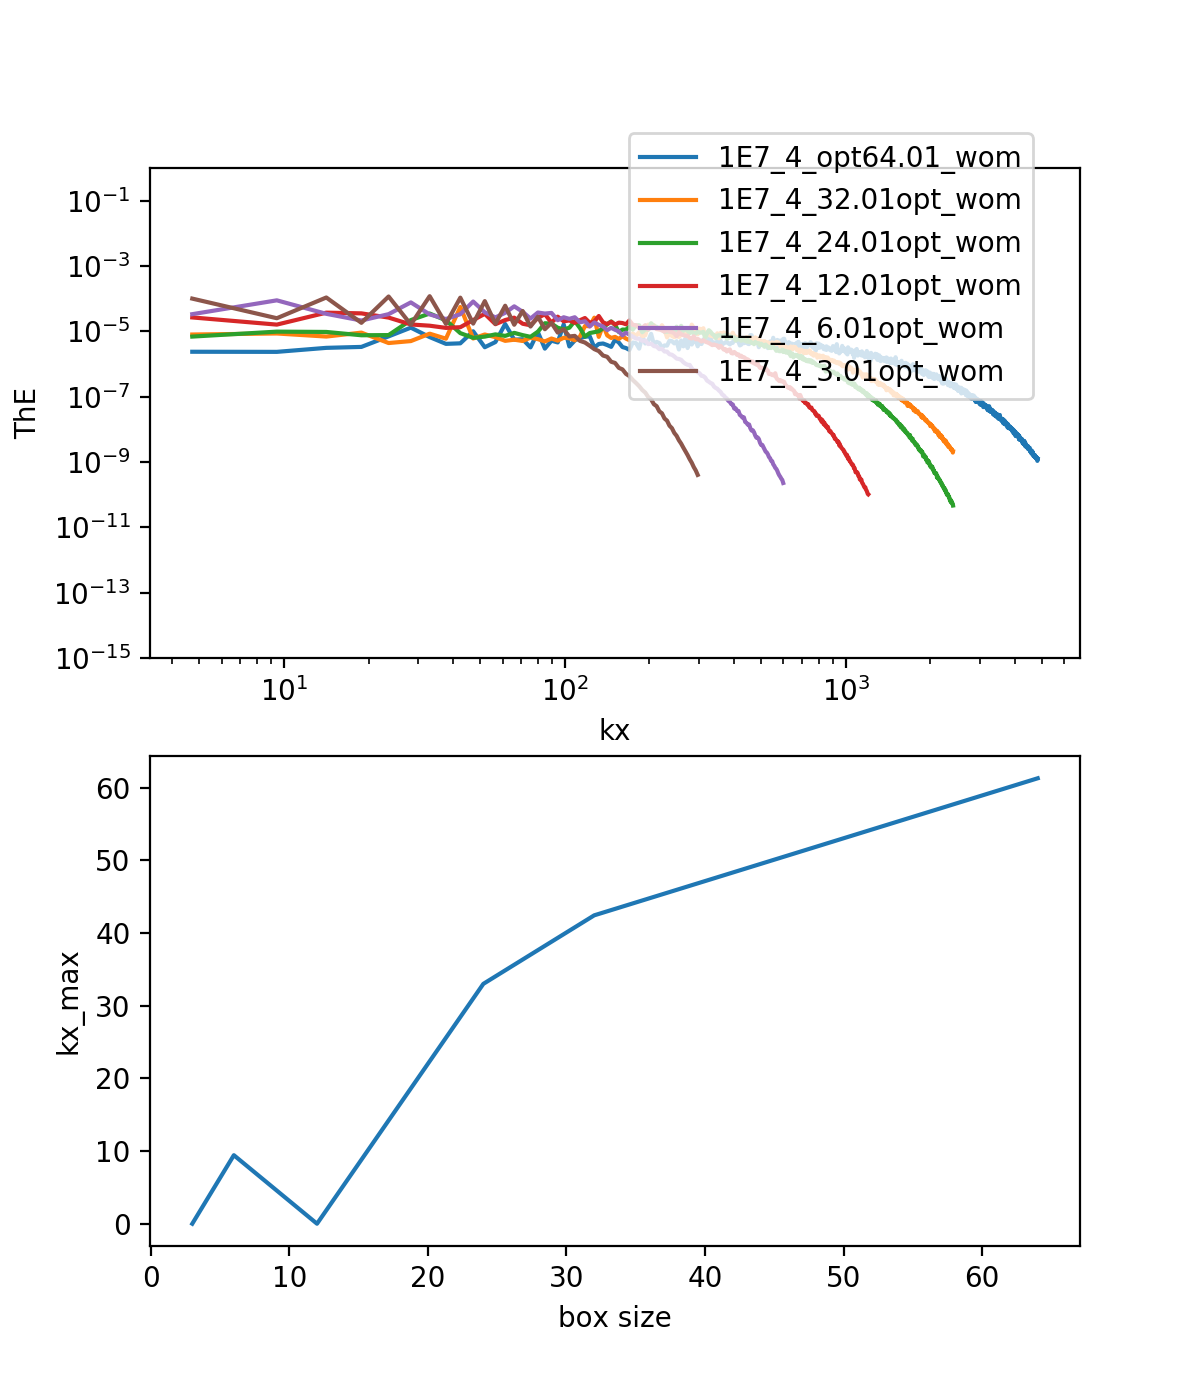
\includegraphics[width=\linewidth]{ThE_1E7_4.png}
  	\caption{ Thermal energy spectra at $Ra = 1E7, Pr =4$ along $y = 0$}
  	\label{fig:fig13}
  \end{figure}

\begin{figure}[!htb]
	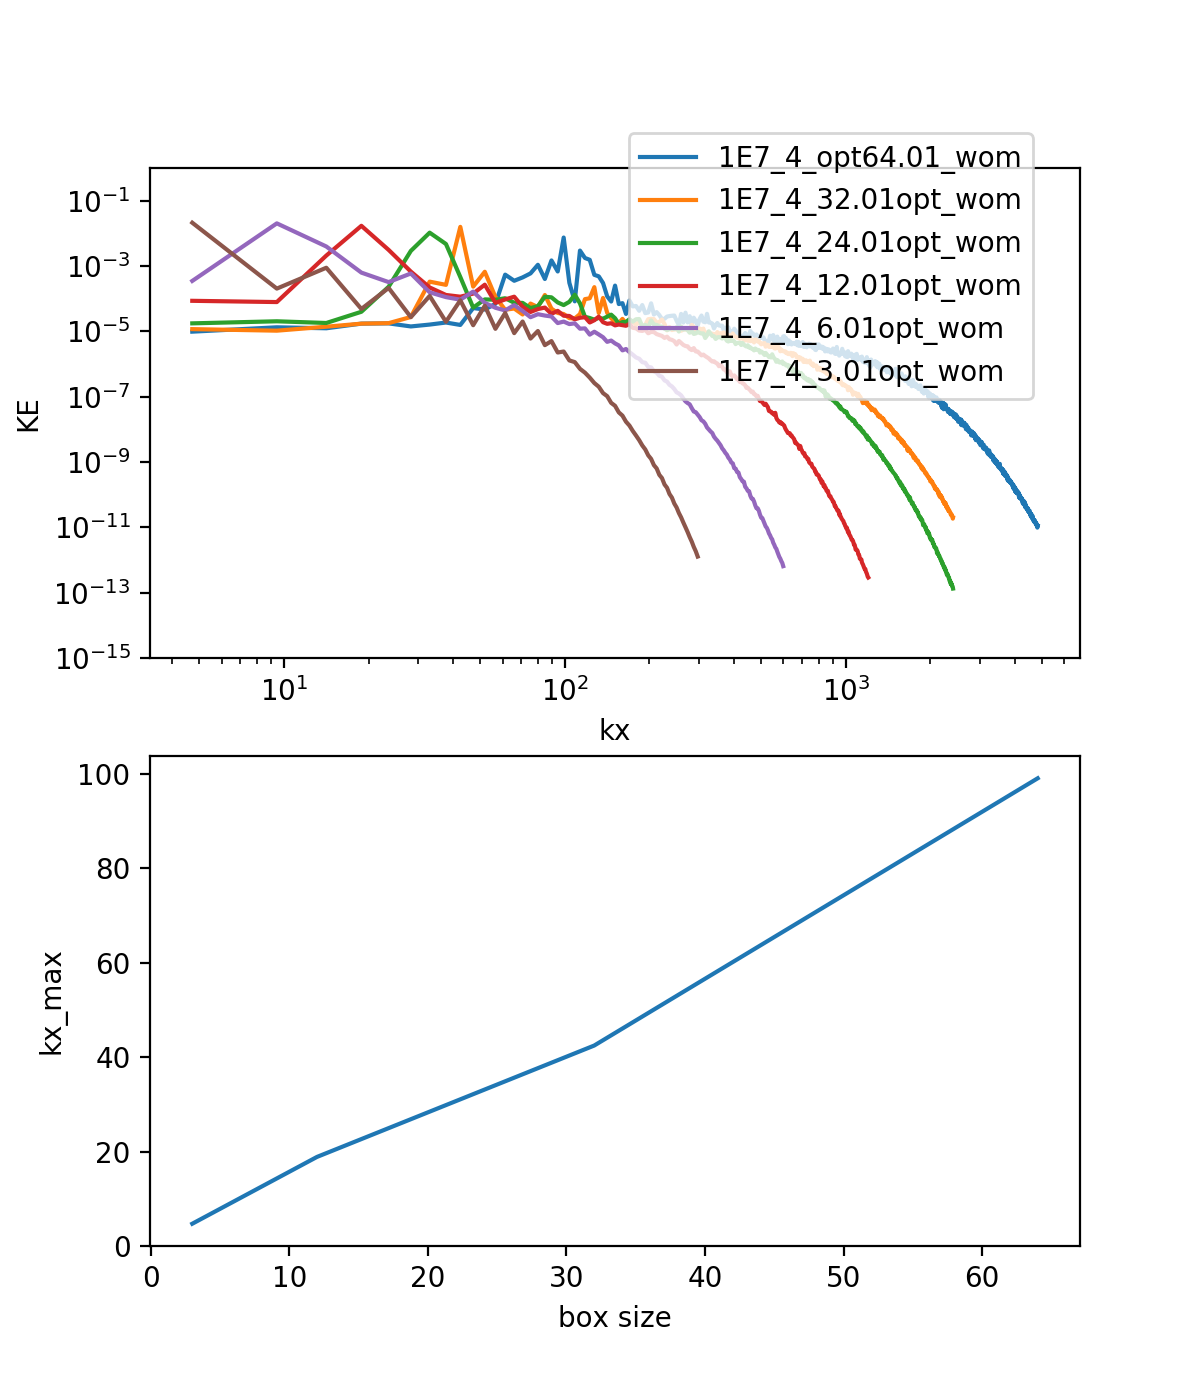
\includegraphics[width=\linewidth]{KE_1E7_4.png}
	\caption{ Kinetic energy spectra at $Ra = 1E7, Pr =4$ along $y = 0$}
	\label{fig:fig14}
\end{figure}

\begin{figure}[!htb]
	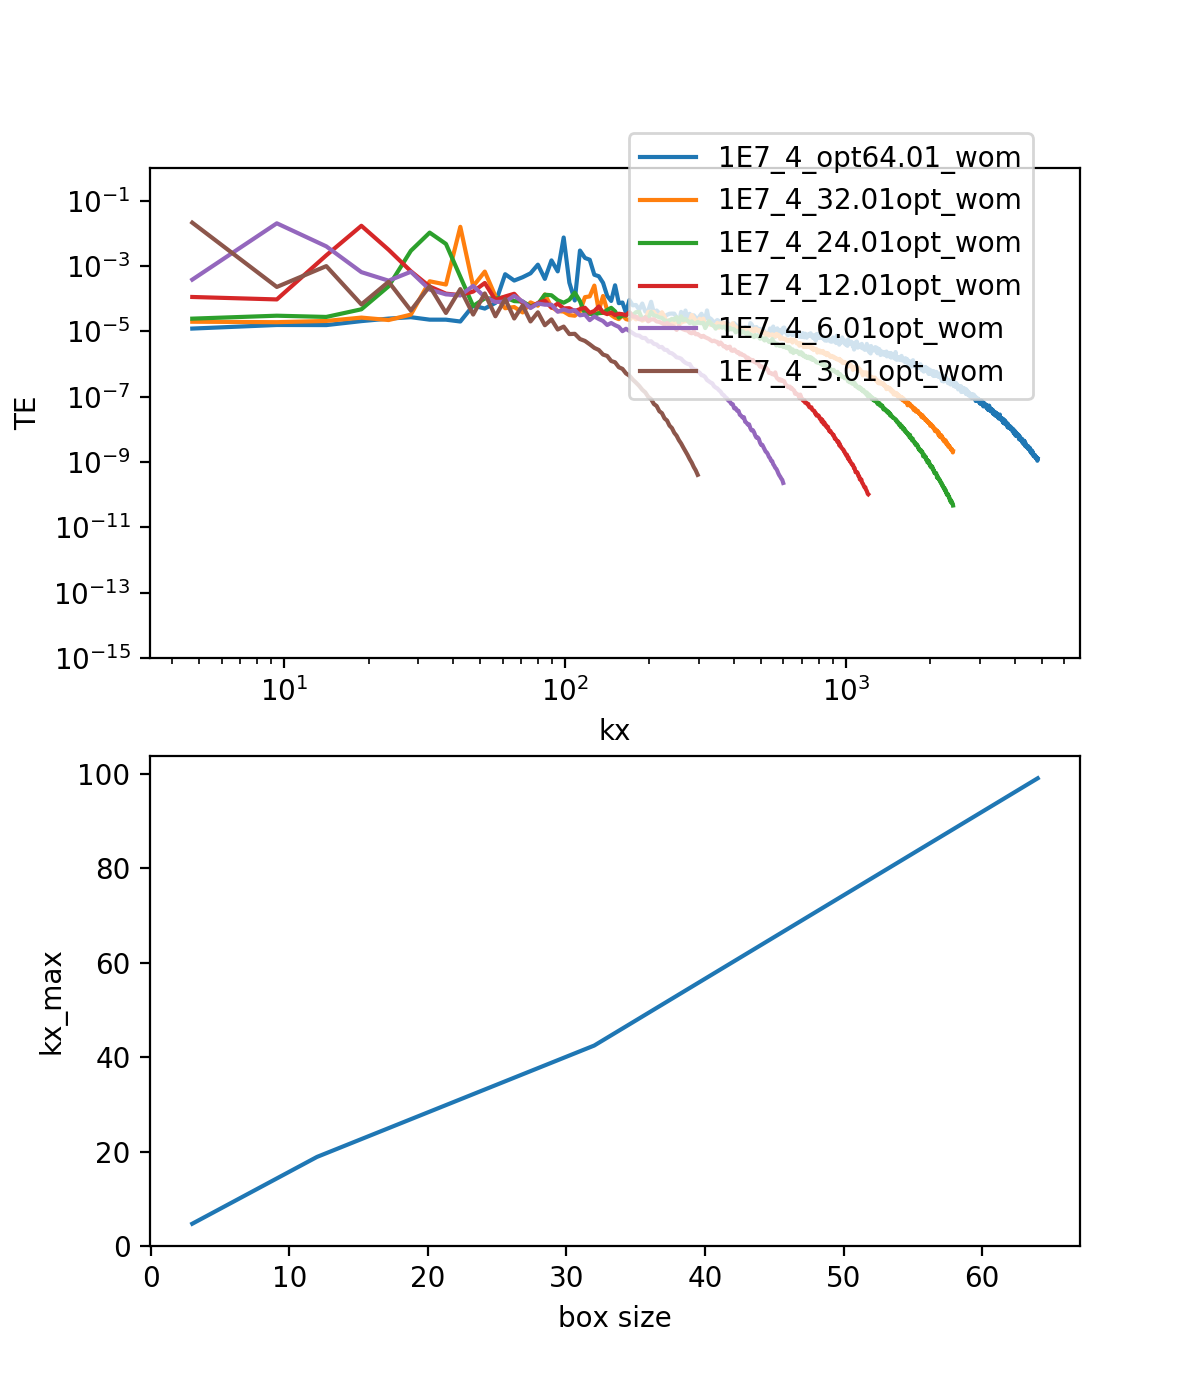
\includegraphics[width=\linewidth]{TE_1E7_4.png}
	\caption{ Total energy spectra at $Ra = 1E7, Pr =4$ along $y = 0$}
	\label{fig:fig15}
\end{figure}

\subsection{Comparison of flow at Ra = 1E7, Pr = 10 in various box sizes}

Simulations were carried out in various boxes where the length is set to be an integral multiple of the optimal box size $(24, 6, 3)$ corresponding to $\alpha_{opt} = alpha = 0.1560021496301813E+002$ at $Ra = 1E7$ and $Pr = 10$. Note that the mean flow is forced to be 0 in all the cases reported.

Figure 16 shows the variation of $Nu$ with time for the different cases and the variation in average $Nu$ with box size is shown in Figure 17. 

     \begin{figure}[!htb]
     	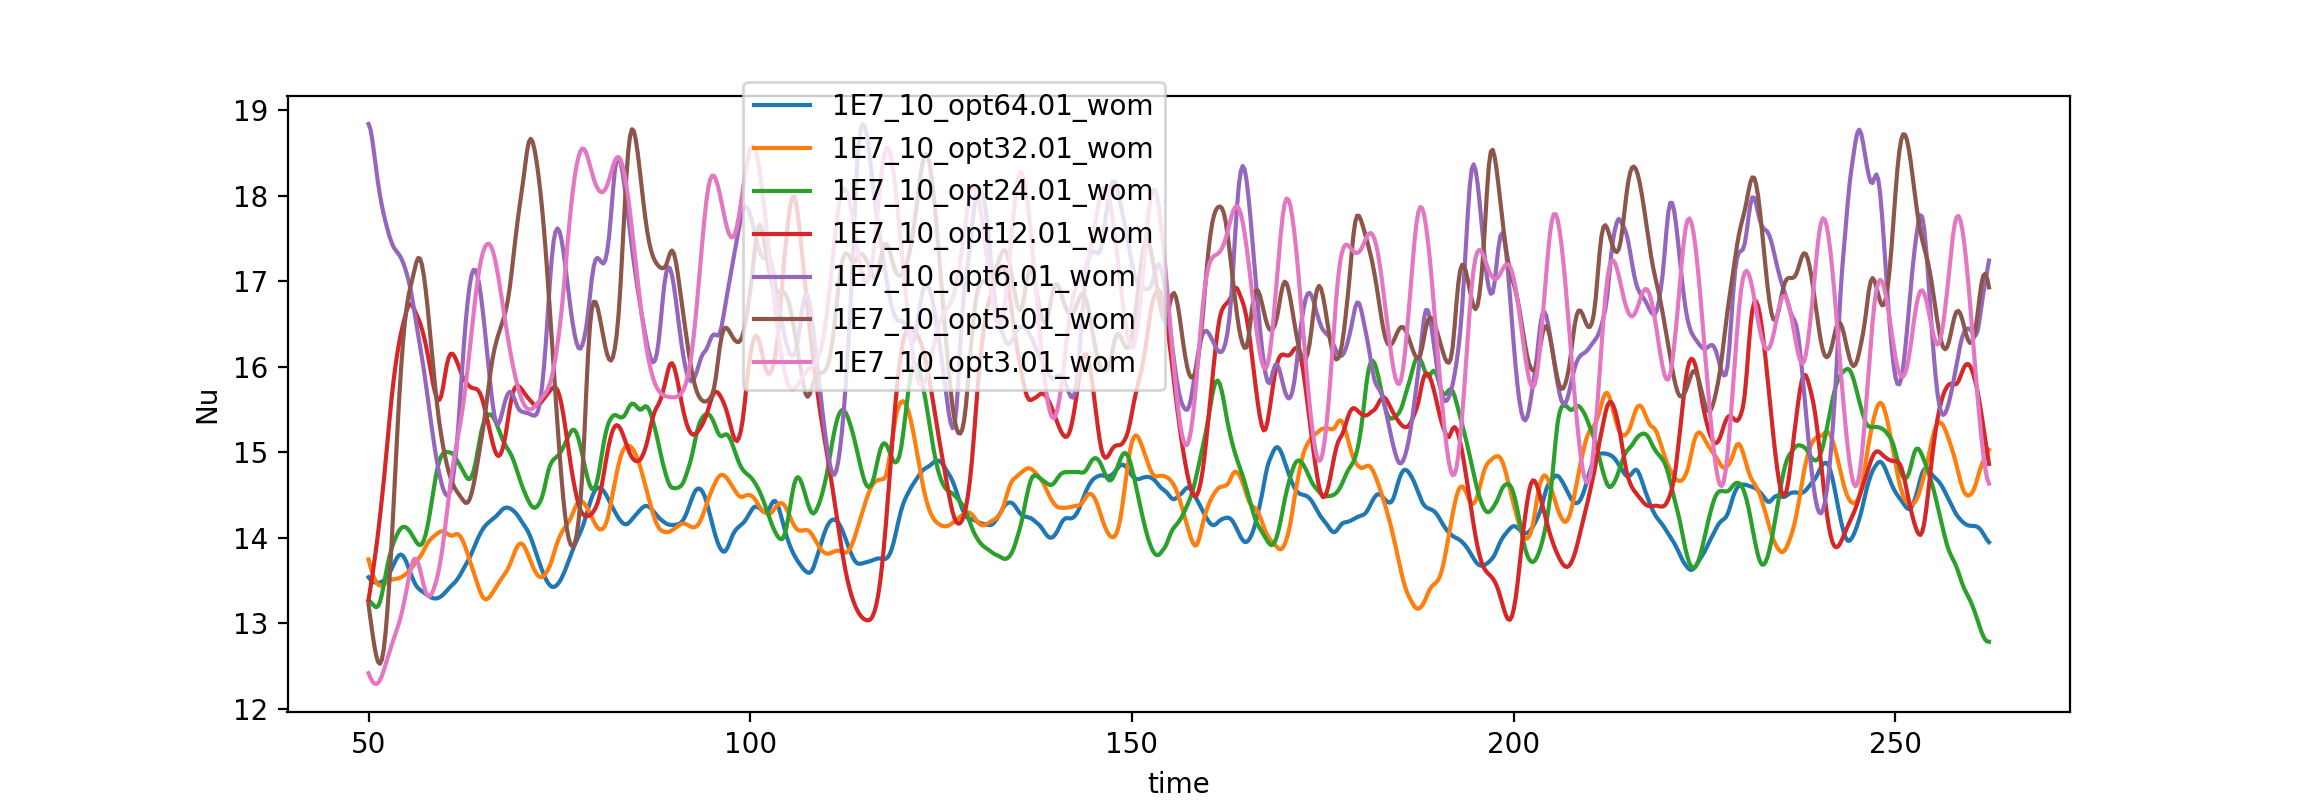
\includegraphics[width=\linewidth]{Nu_1E7_10.png}
     	\caption{$Nu$ variation with time at $Pr = 10, Ra = 1E7$ in various box sizes.}
     	\label{fig:fig16}
     \end{figure} 
     
     \begin{figure}[!htb]
     	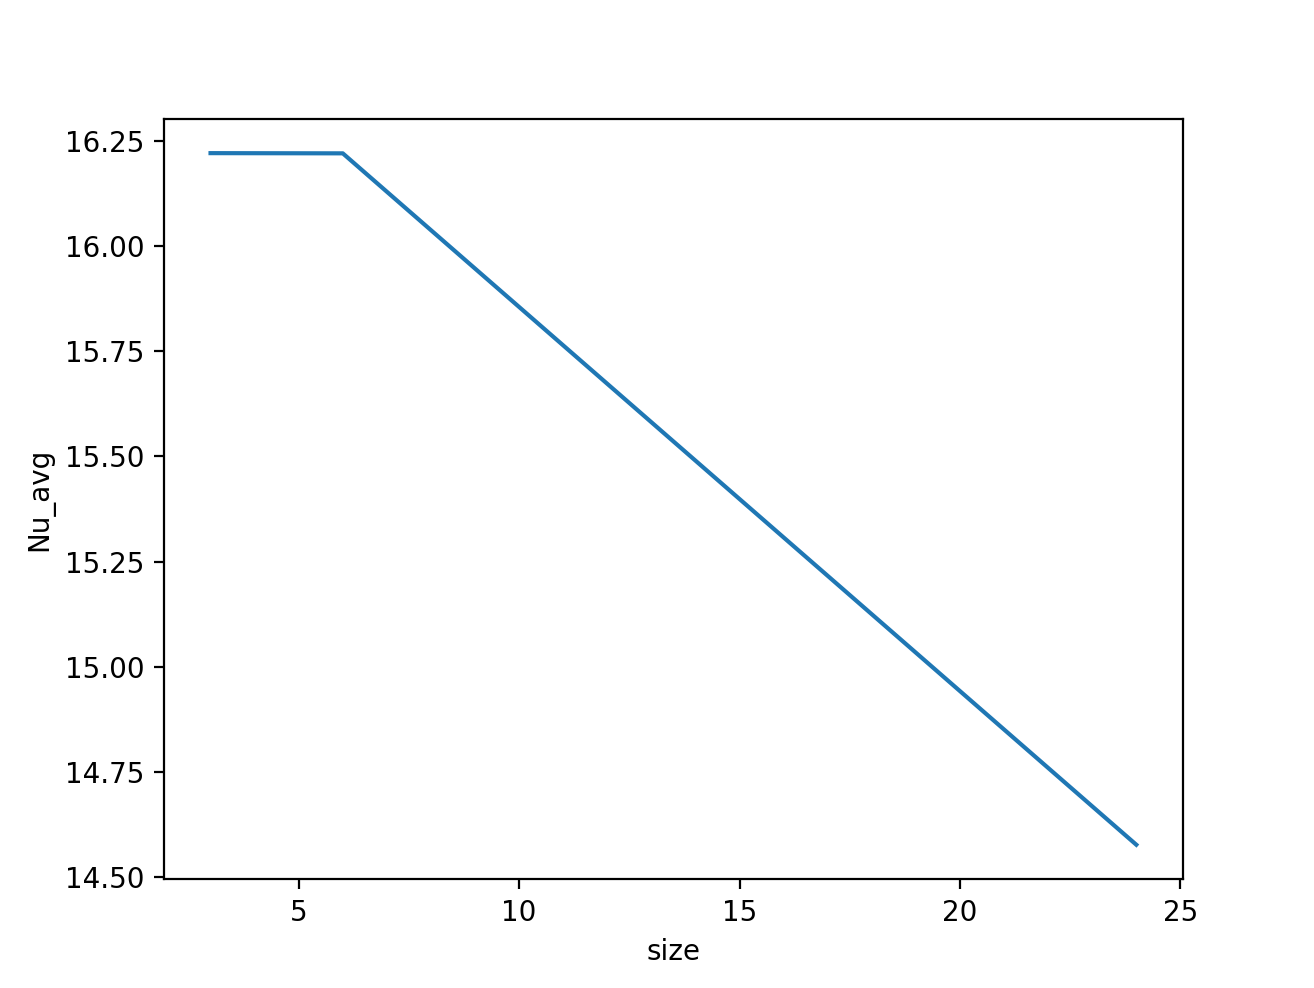
\includegraphics[width=\linewidth]{Nu_avg_1E7_10.png}
     	\caption{$Nu_{avg}$ variation with box size for $Pr = 10, Ra = 1E7$.}
     	\label{fig:fig17}
     \end{figure} 
     
     The contours of $T,u,w$ are plotted in Figures 18-20 for the 3 cases considered. The time is chosen such that the flow has attained a statistically steady state.
     
     \begin{figure}[!htb]
     	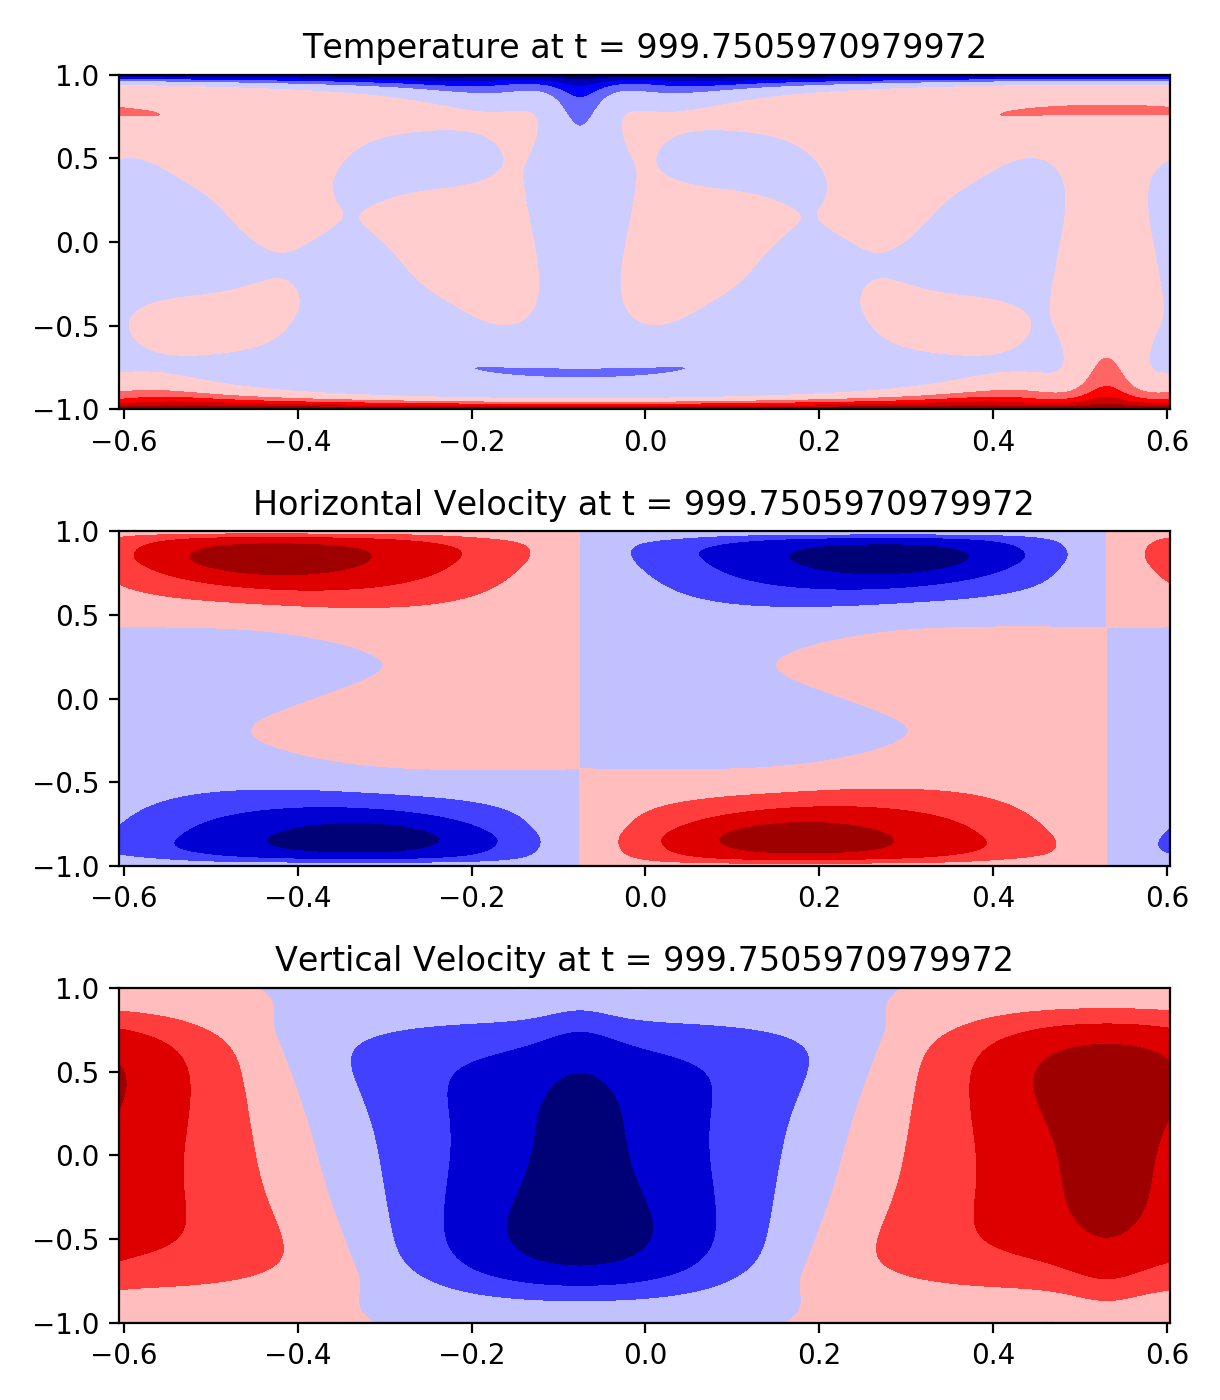
\includegraphics[width=\linewidth]{contours_1E7_10_3.png}
     	\caption{Temperature, horizontal and vertical velocity contours for $Ra = 1E7, Pr =10, l_b = 3* l_{opt} $ }
     	\label{fig:fig18}
     \end{figure}
     
     \clearpage
     
     \begin{figure}[!htb]
     	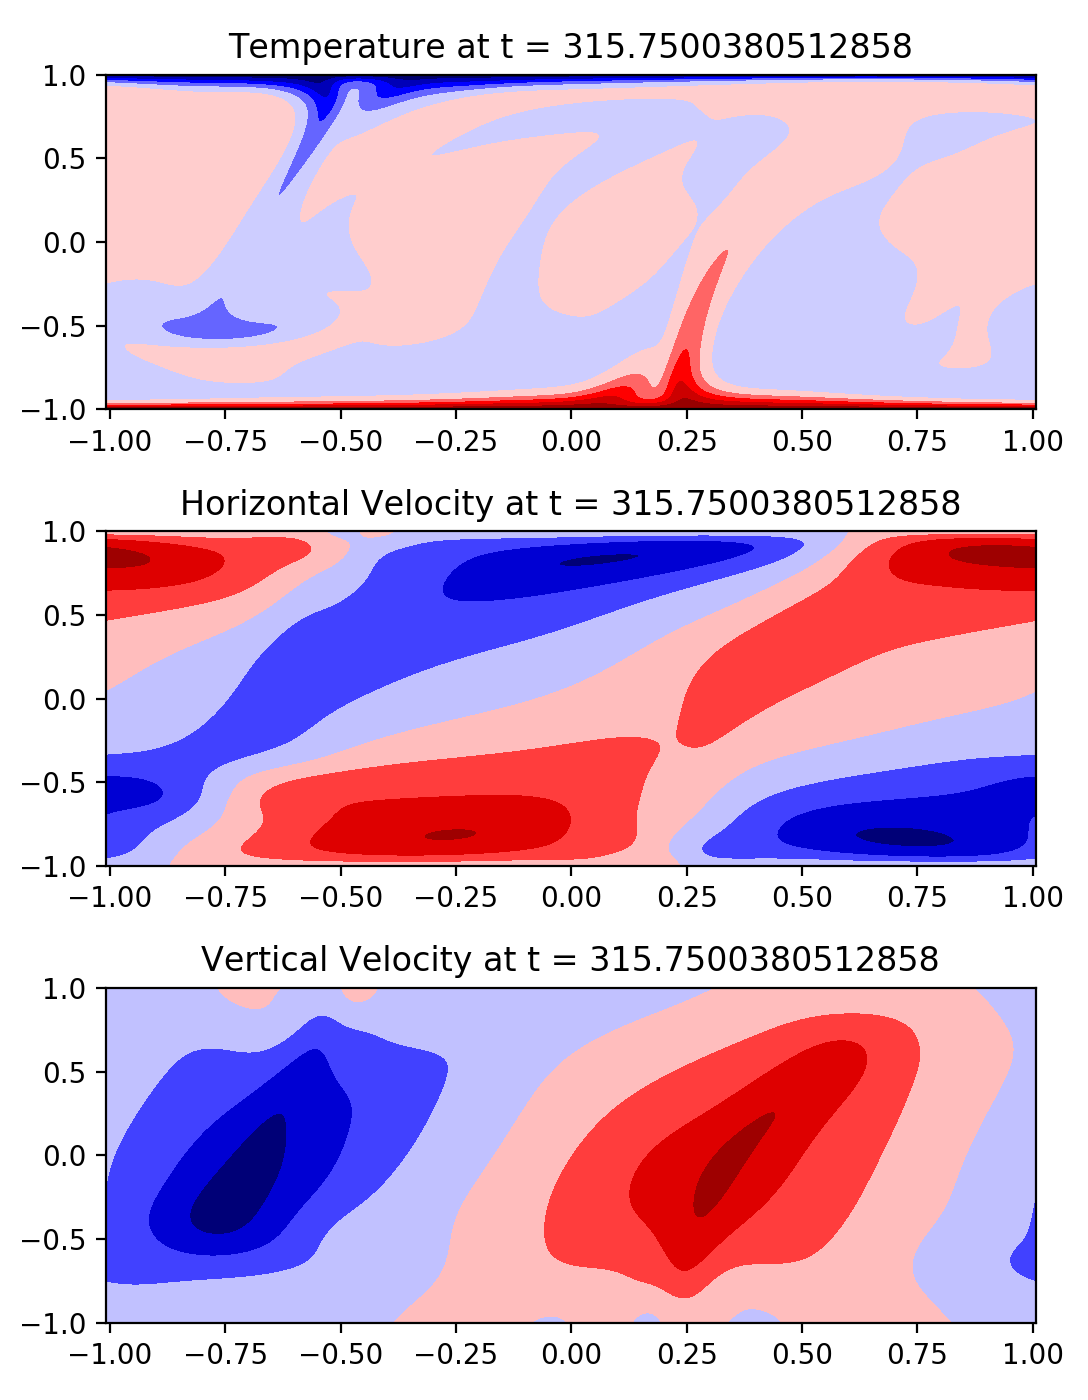
\includegraphics[width=\linewidth]{contours_1E7_10_5.png}
     	\caption{Temperature, horizontal and vertical velocity contours for $Ra = 1E7, Pr =10, l_b = 5* l_{opt} $ }
     	\label{fig:fig20}
     \end{figure}
     
     
     \begin{figure}[!htb]
     	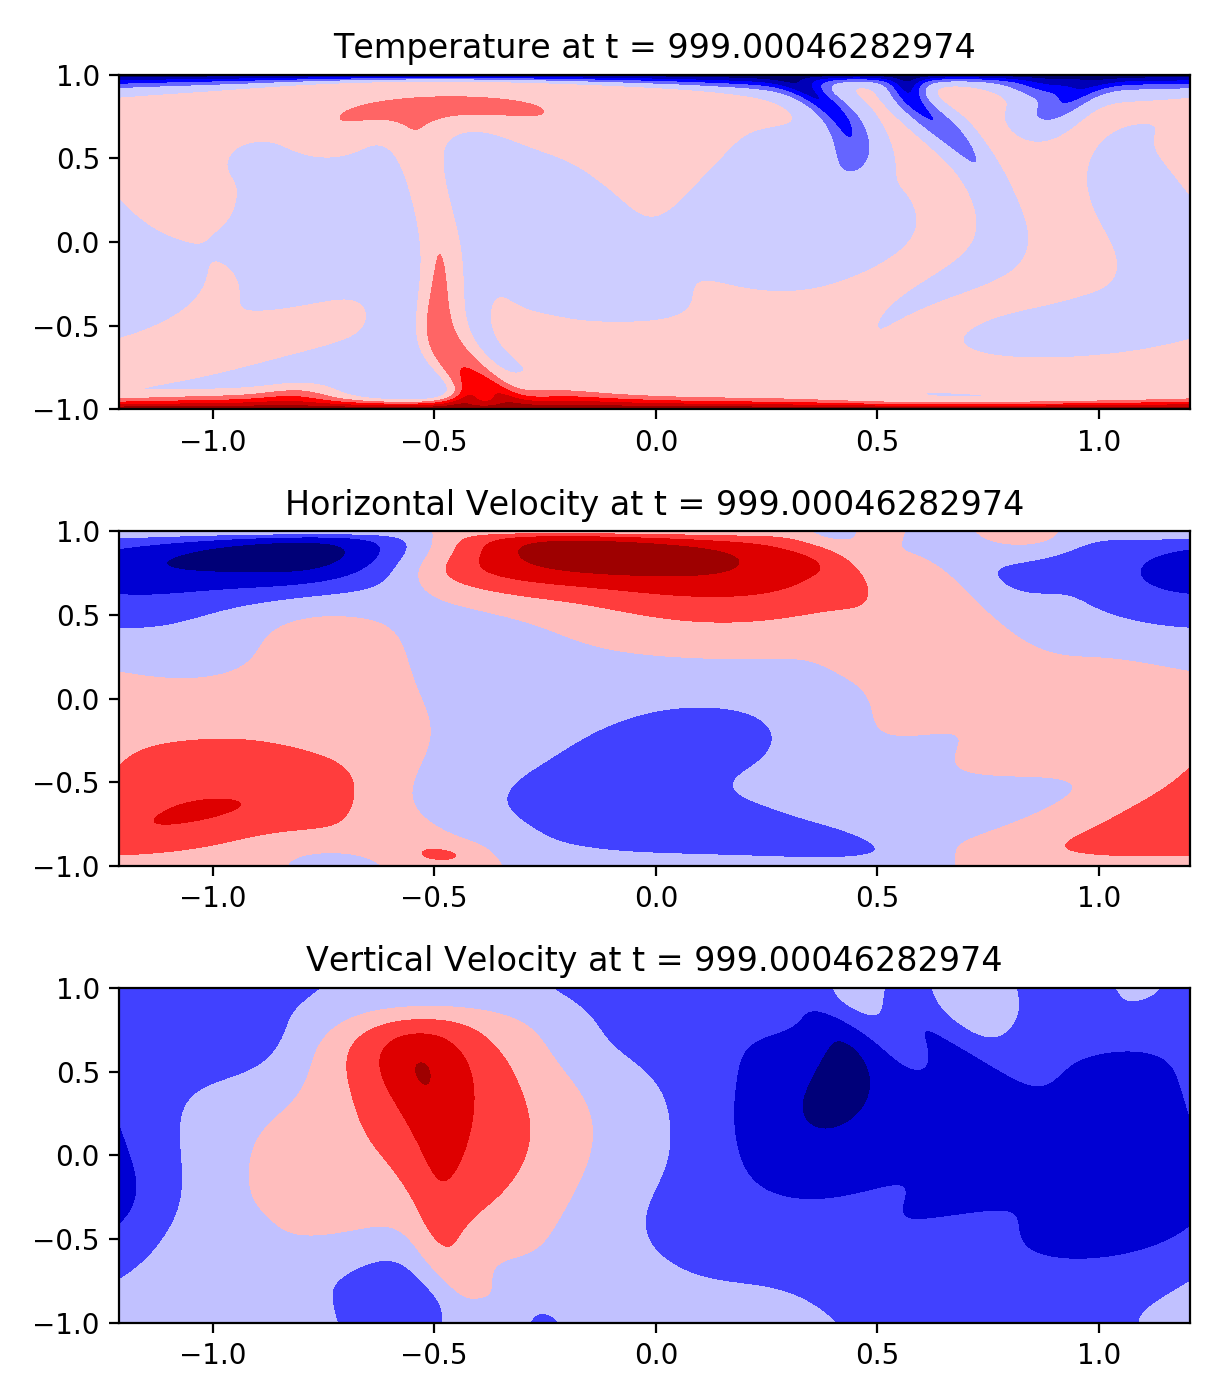
\includegraphics[width=\linewidth]{contours_1E7_10_6.png}
     	\caption{Temperature, horizontal and vertical velocity contours for $Ra = 1E7, Pr =10, l_b = 6* l_{opt} $ }
     	\label{fig:fig20}
     \end{figure}
     
     \begin{figure}[!htb]
     	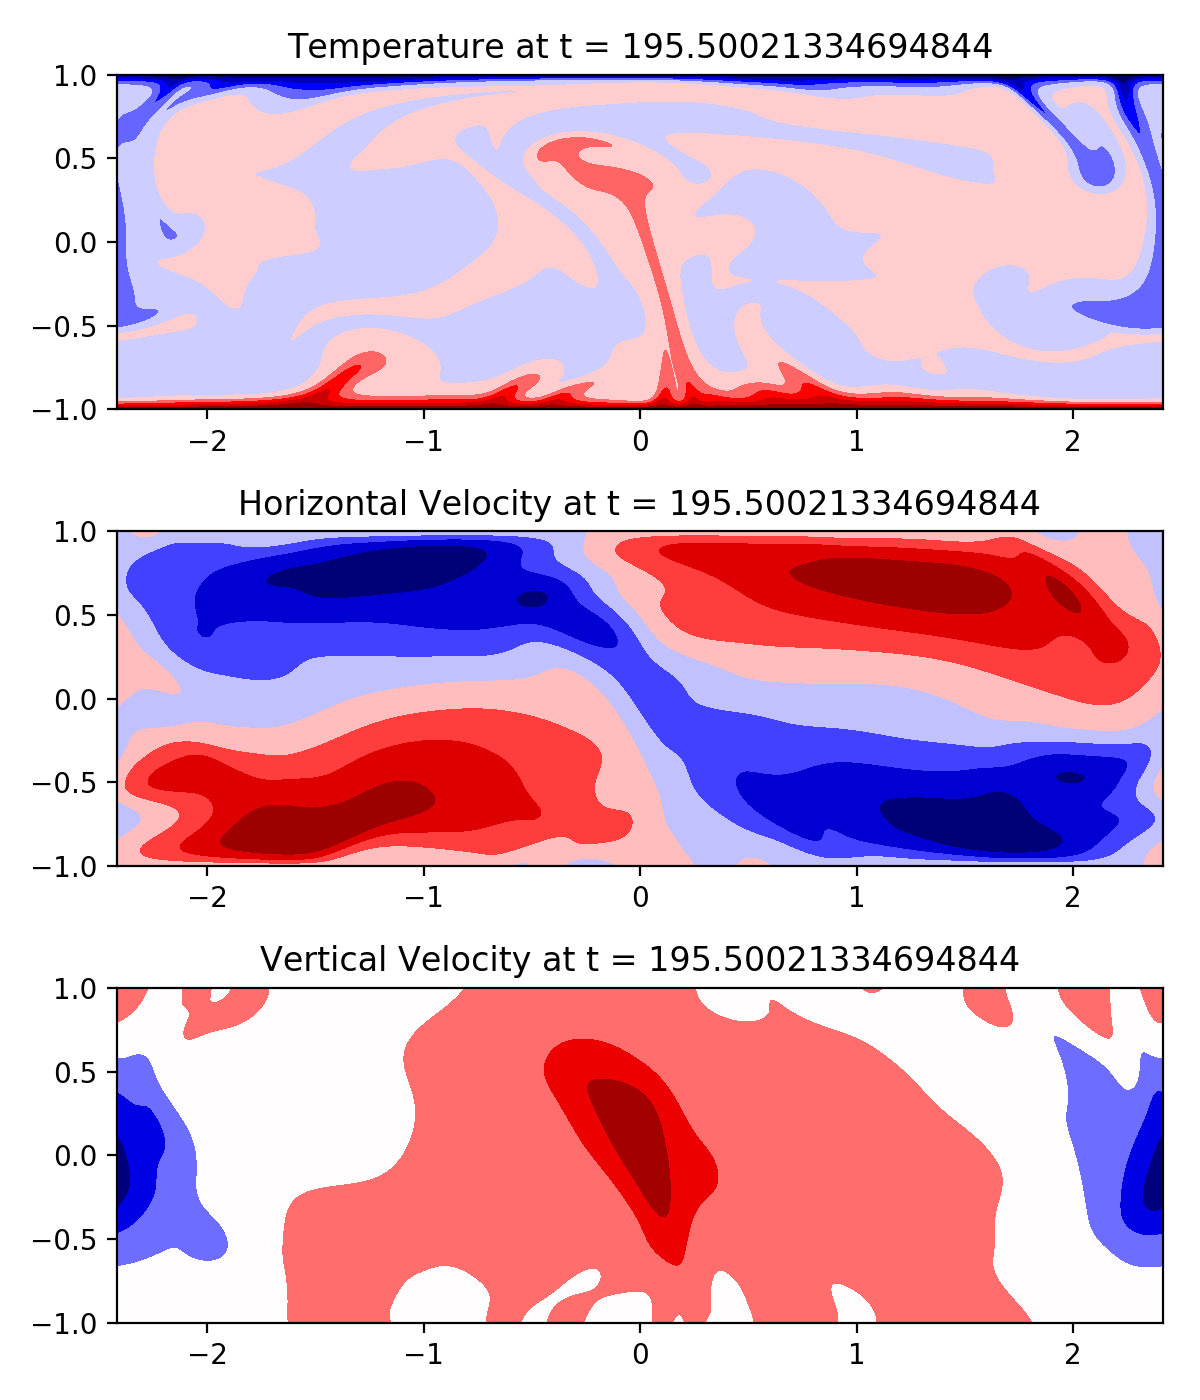
\includegraphics[width=\linewidth]{contours_1E7_10_12.png}
     	\caption{Temperature, horizontal and vertical velocity contours for $Ra = 1E7, Pr =10, l_b = 12* l_{opt} $ }
     	\label{fig:fig20}
     \end{figure}
     
     
     \begin{figure}[!htb]
     	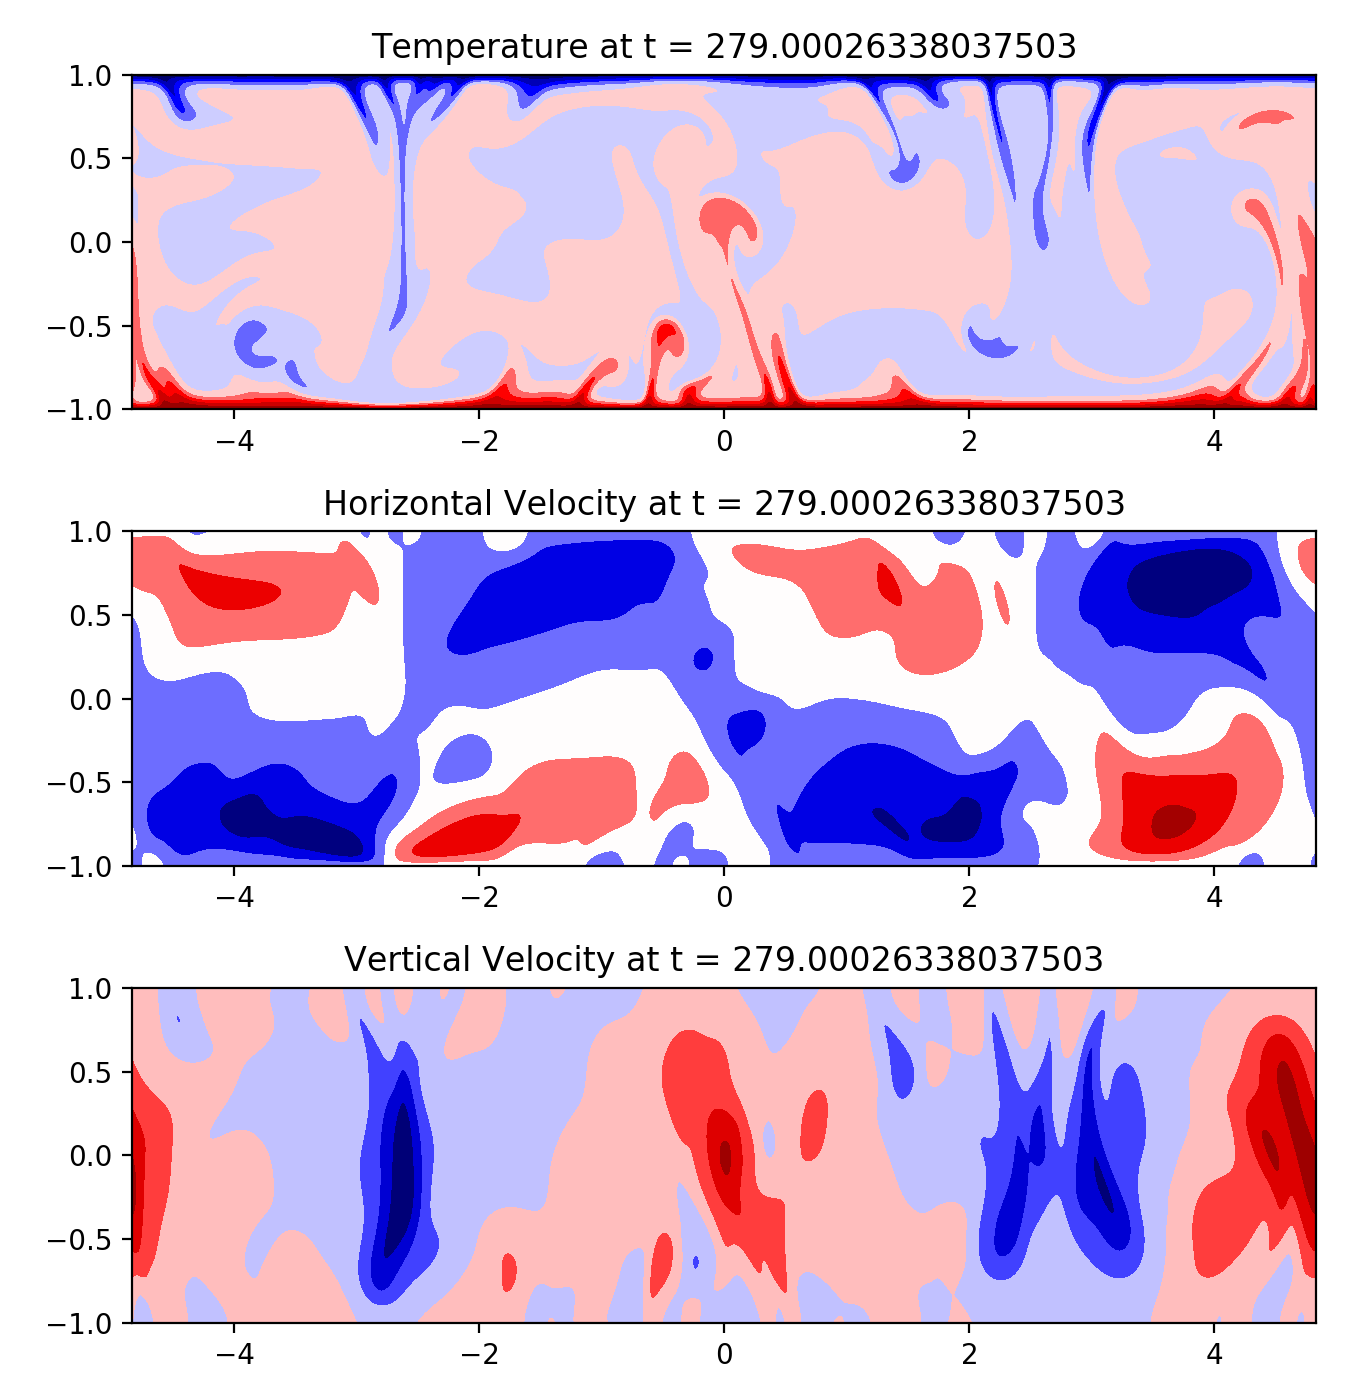
\includegraphics[width=\linewidth]{contours_1E7_10_24.png}
     	\caption{Temperature, horizontal and vertical velocity contours for $Ra = 1E7, Pr =10, l_b = 24* l_{opt} $ }
     	\label{fig:fig21}
     \end{figure}
     
       \begin{figure}[!htb]
       	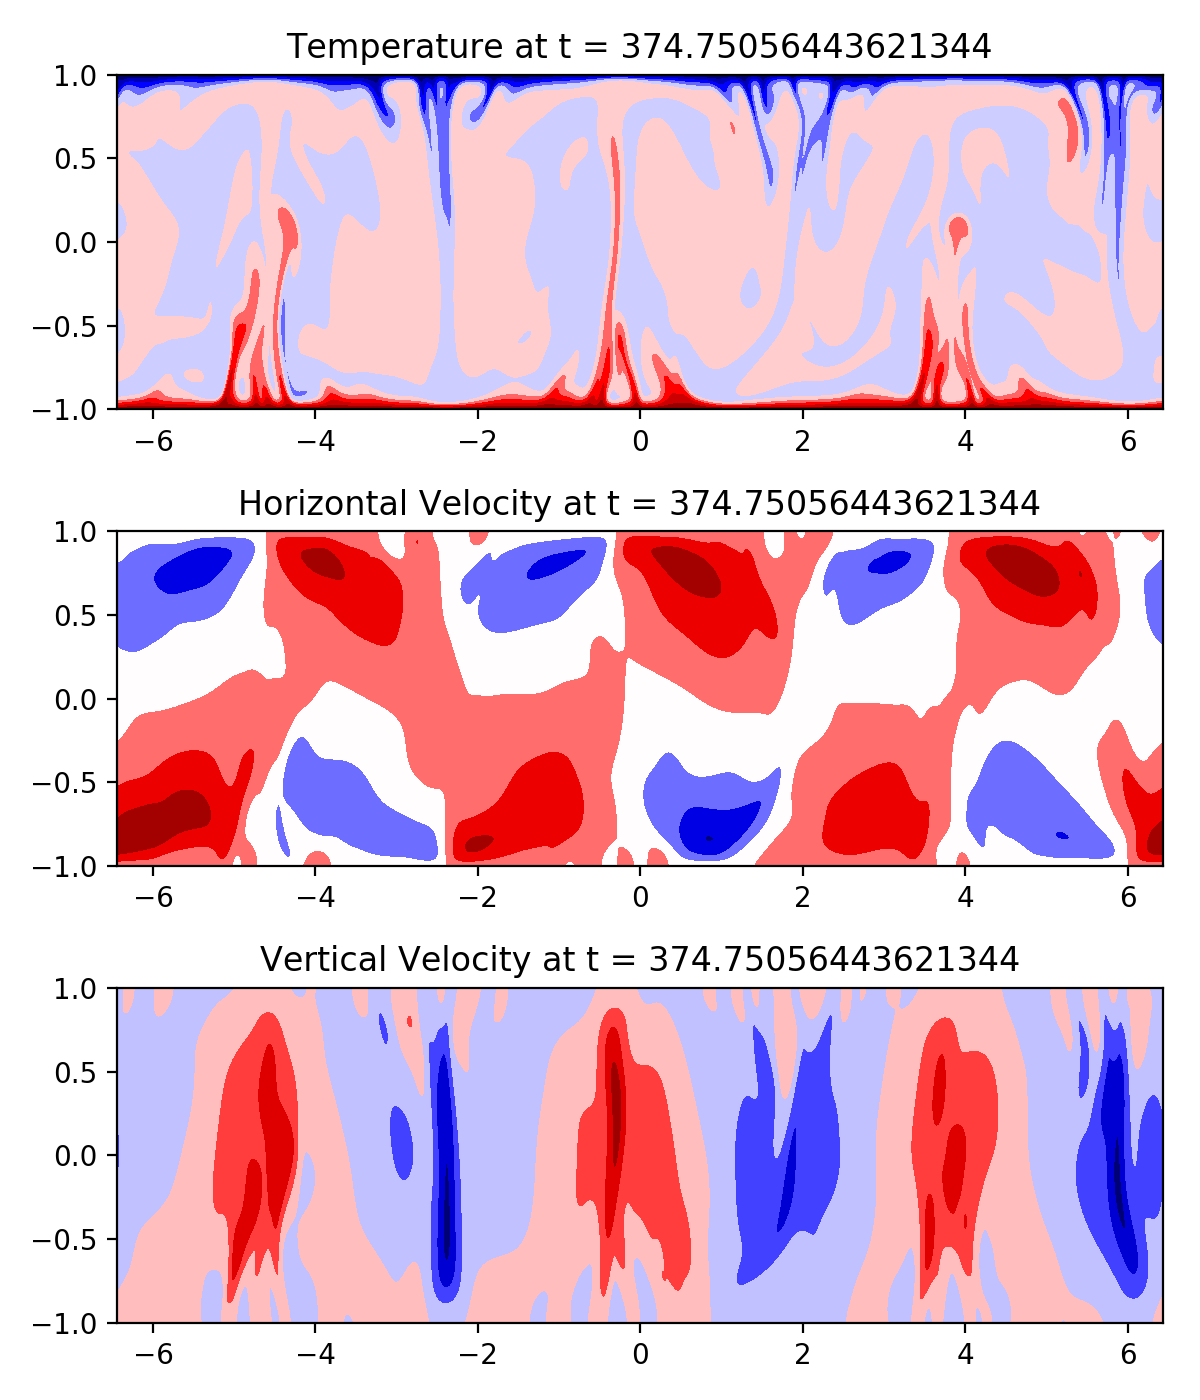
\includegraphics[width=\linewidth]{contours_1E7_10_32.png}
       	\caption{Temperature, horizontal and vertical velocity contours for $Ra = 1E7, Pr =10, l_b = 32* l_{opt} $ }
       	\label{fig:fig21}
       \end{figure}
       
        \begin{figure}[!htb]
        	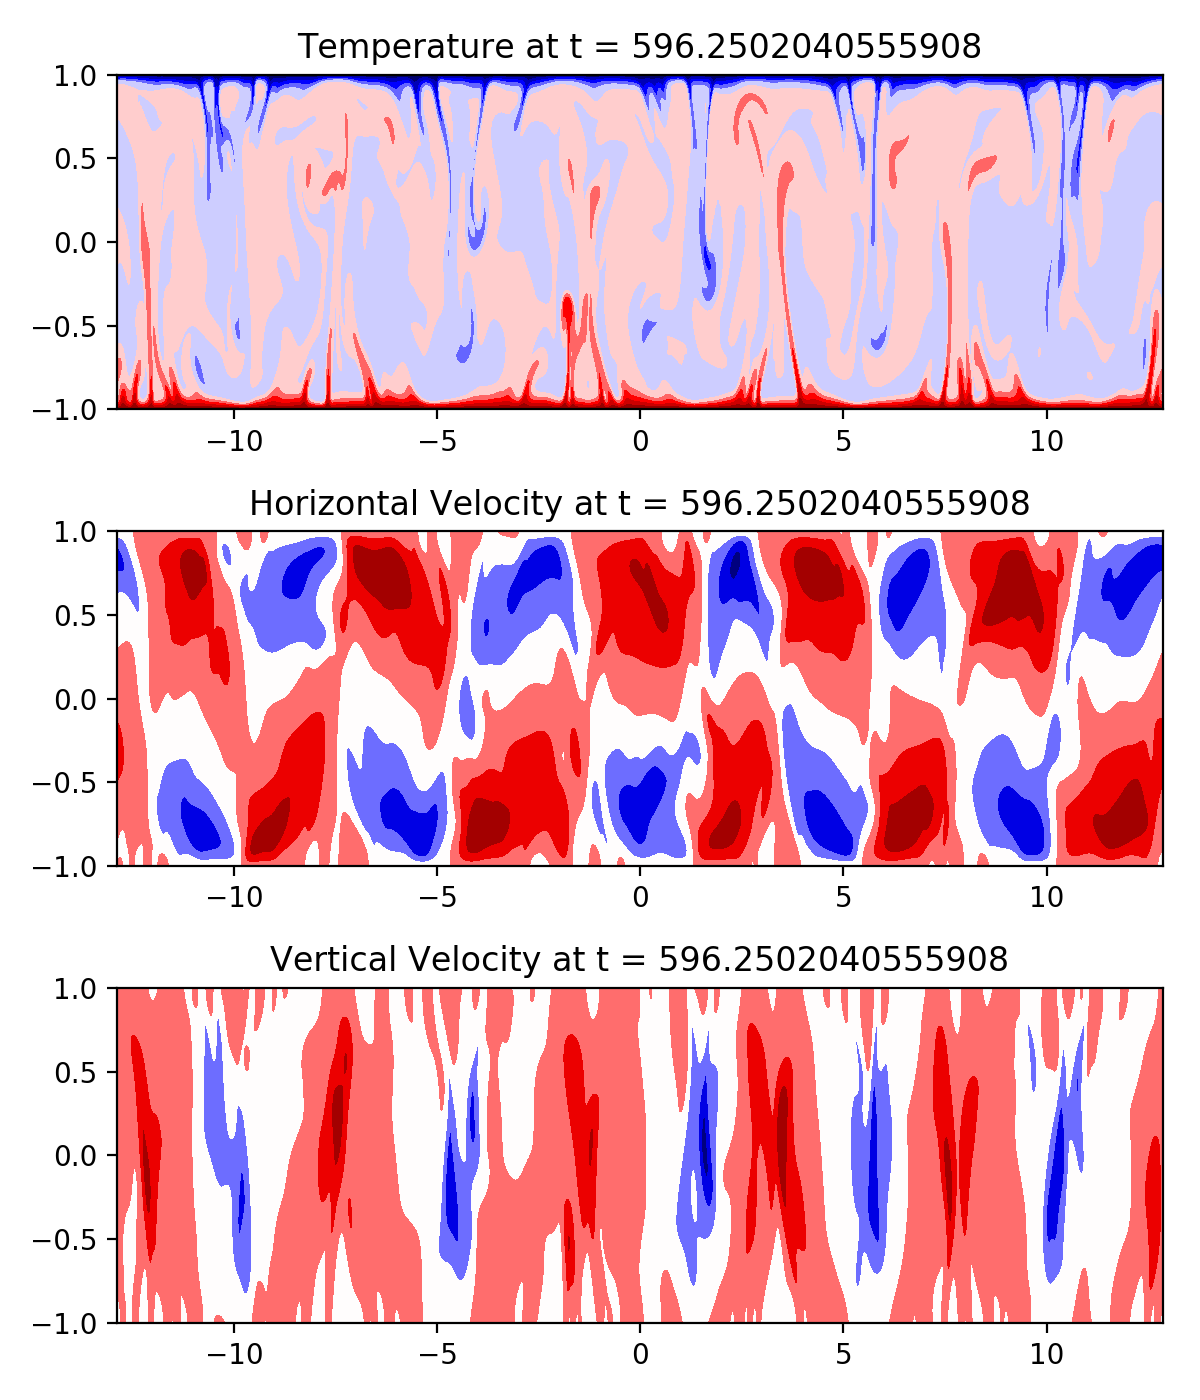
\includegraphics[width=\linewidth]{contours_1E7_10_64.png}
        	\caption{Temperature, horizontal and vertical velocity contours for $Ra = 1E7, Pr =10, l_b = 64* l_{opt} $ }
        	\label{fig:fig21}
        \end{figure}
     
     A comparison of the energy spectra for the various cases are shown in Figures 22-24. The energy spectra is plotted along $y = 0$. 
     
      \begin{figure}[!htb]
      	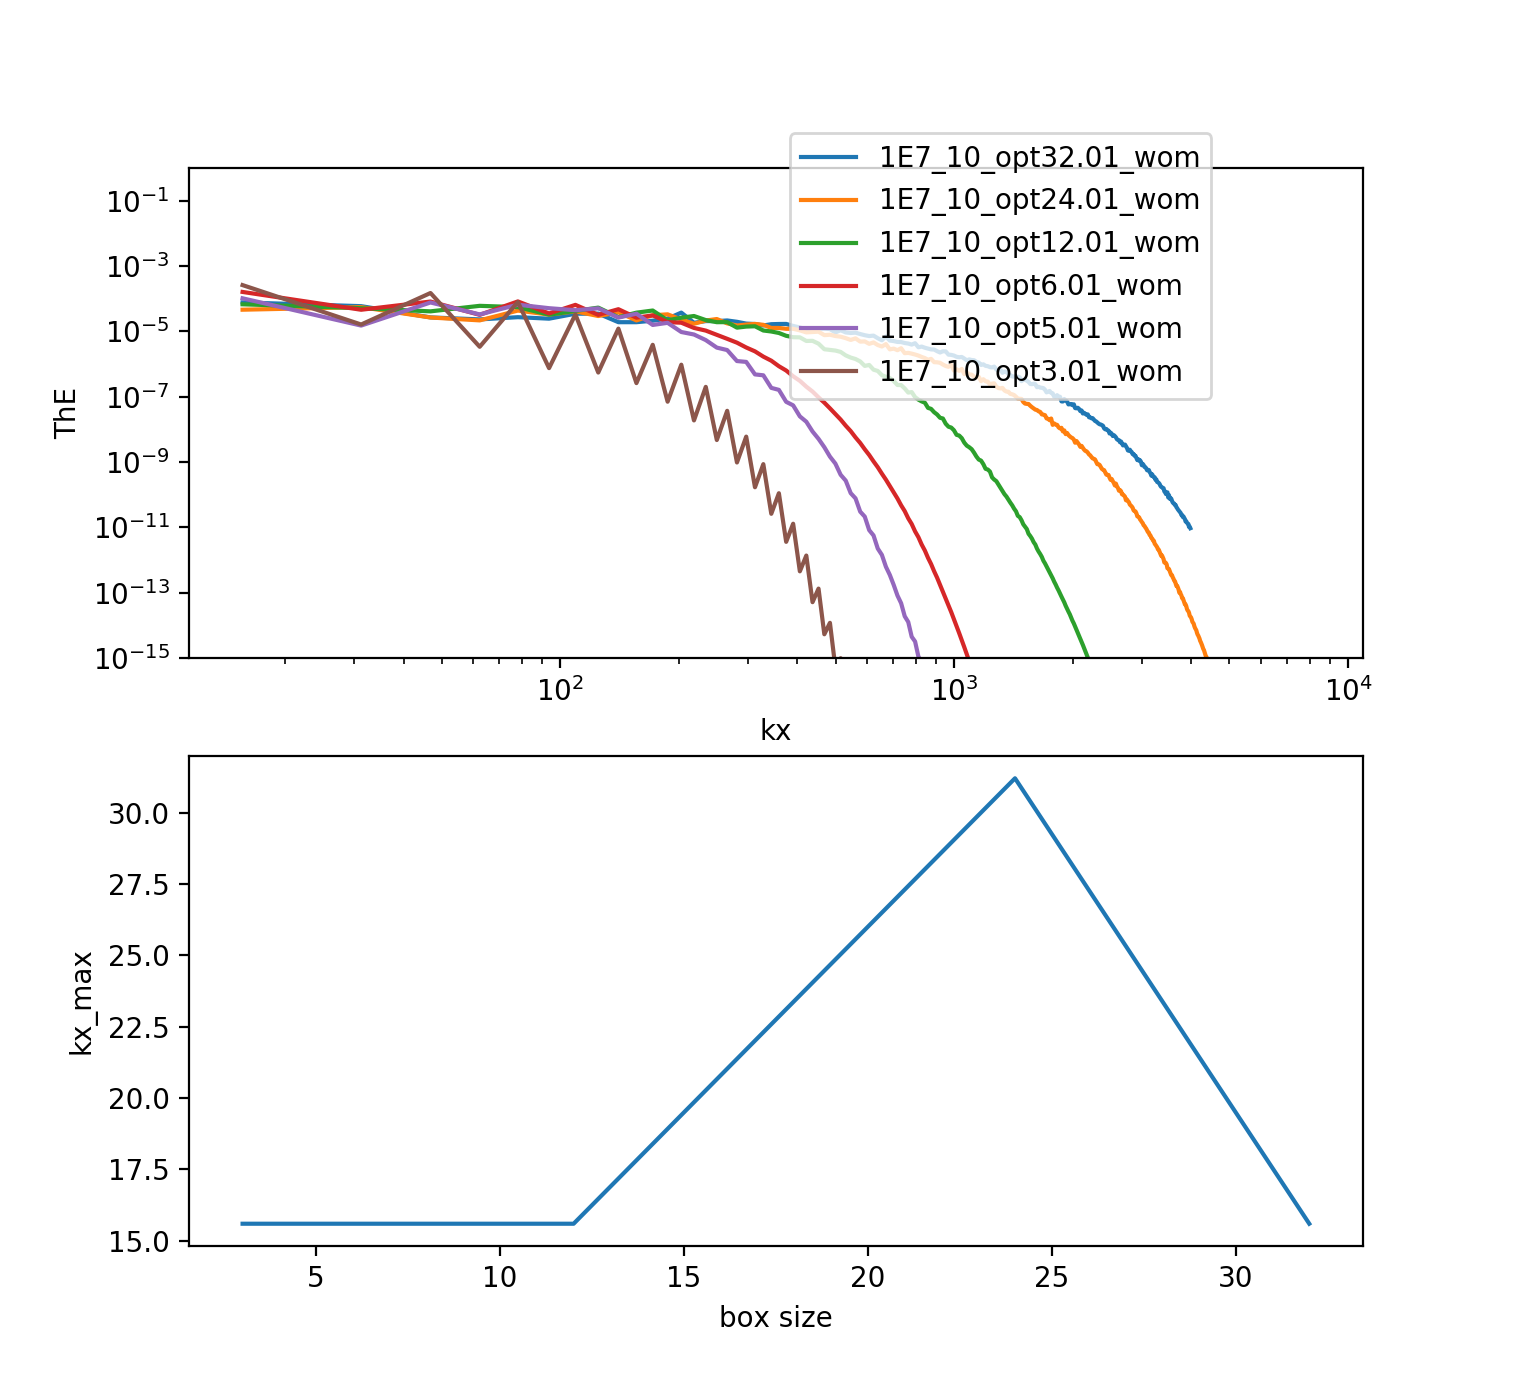
\includegraphics[width=\linewidth]{ThE_1E7_10.png}
      	\caption{ Thermal energy spectra at $Ra = 1E7, Pr =10$ along $y = 0$}
      	\label{fig:fig22}
      \end{figure}
      
     
     \begin{figure}[!htb]
     	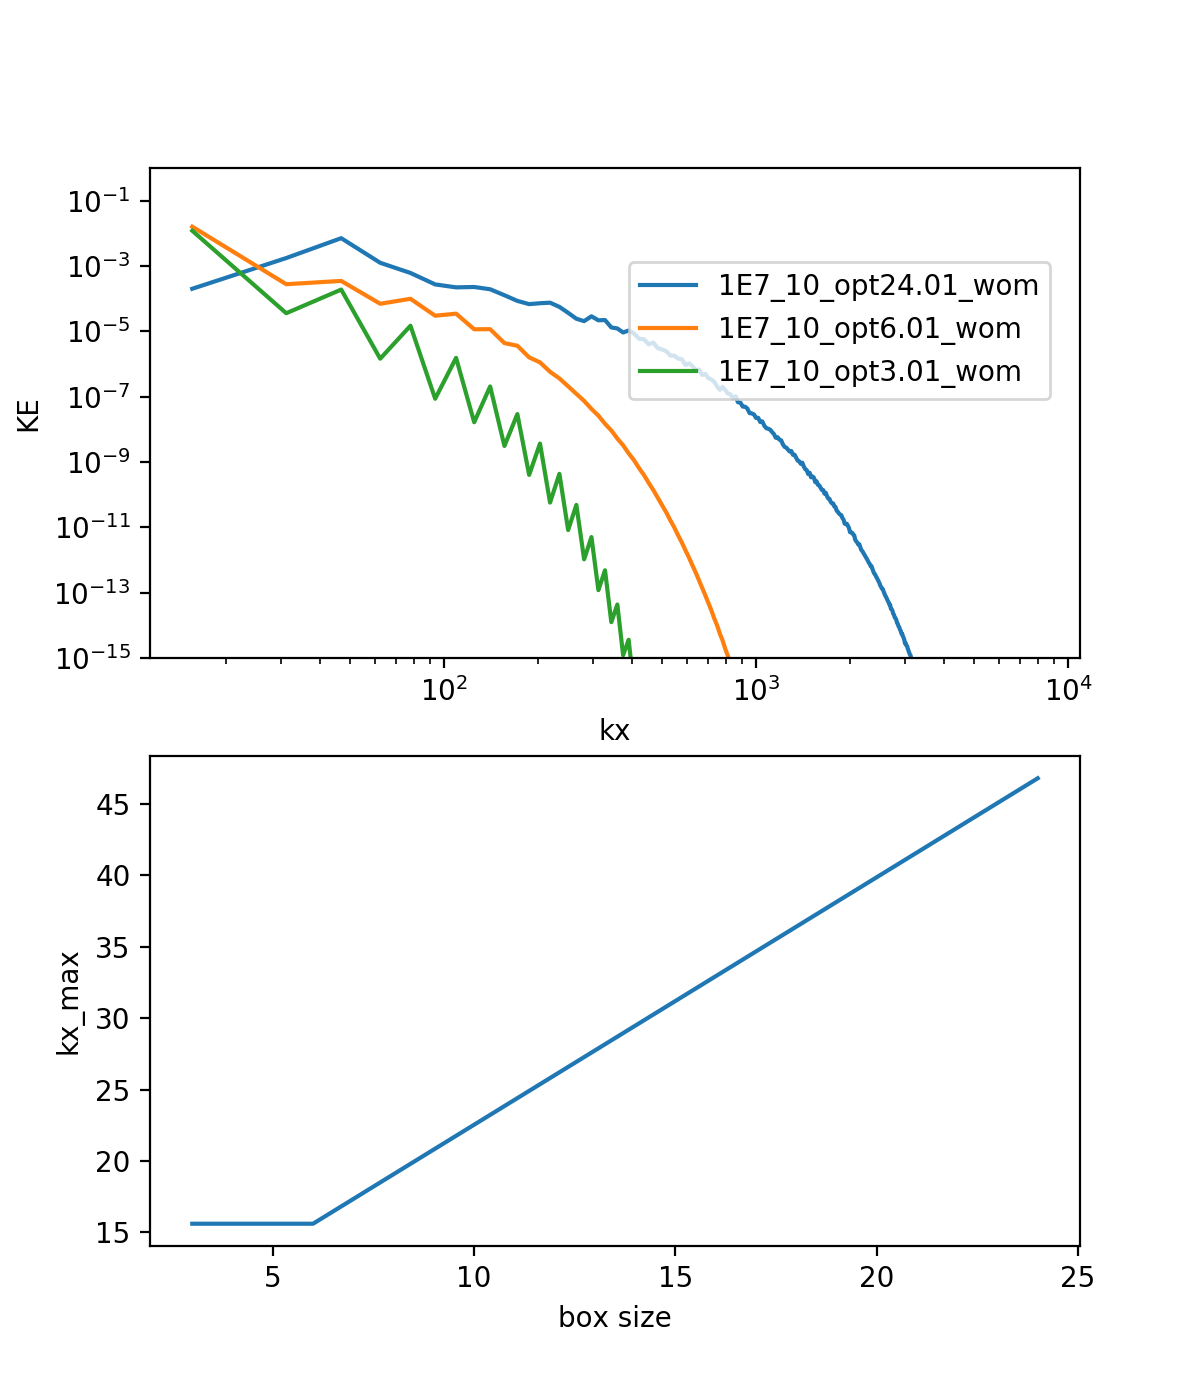
\includegraphics[width=\linewidth]{KE_1E7_10.png}
     	\caption{ Kinetic energy spectra at $Ra = 1E7, Pr =10$ along $y = 0$}
     	\label{fig:fig23}
     \end{figure}
     
      \begin{figure}[!htb]
      	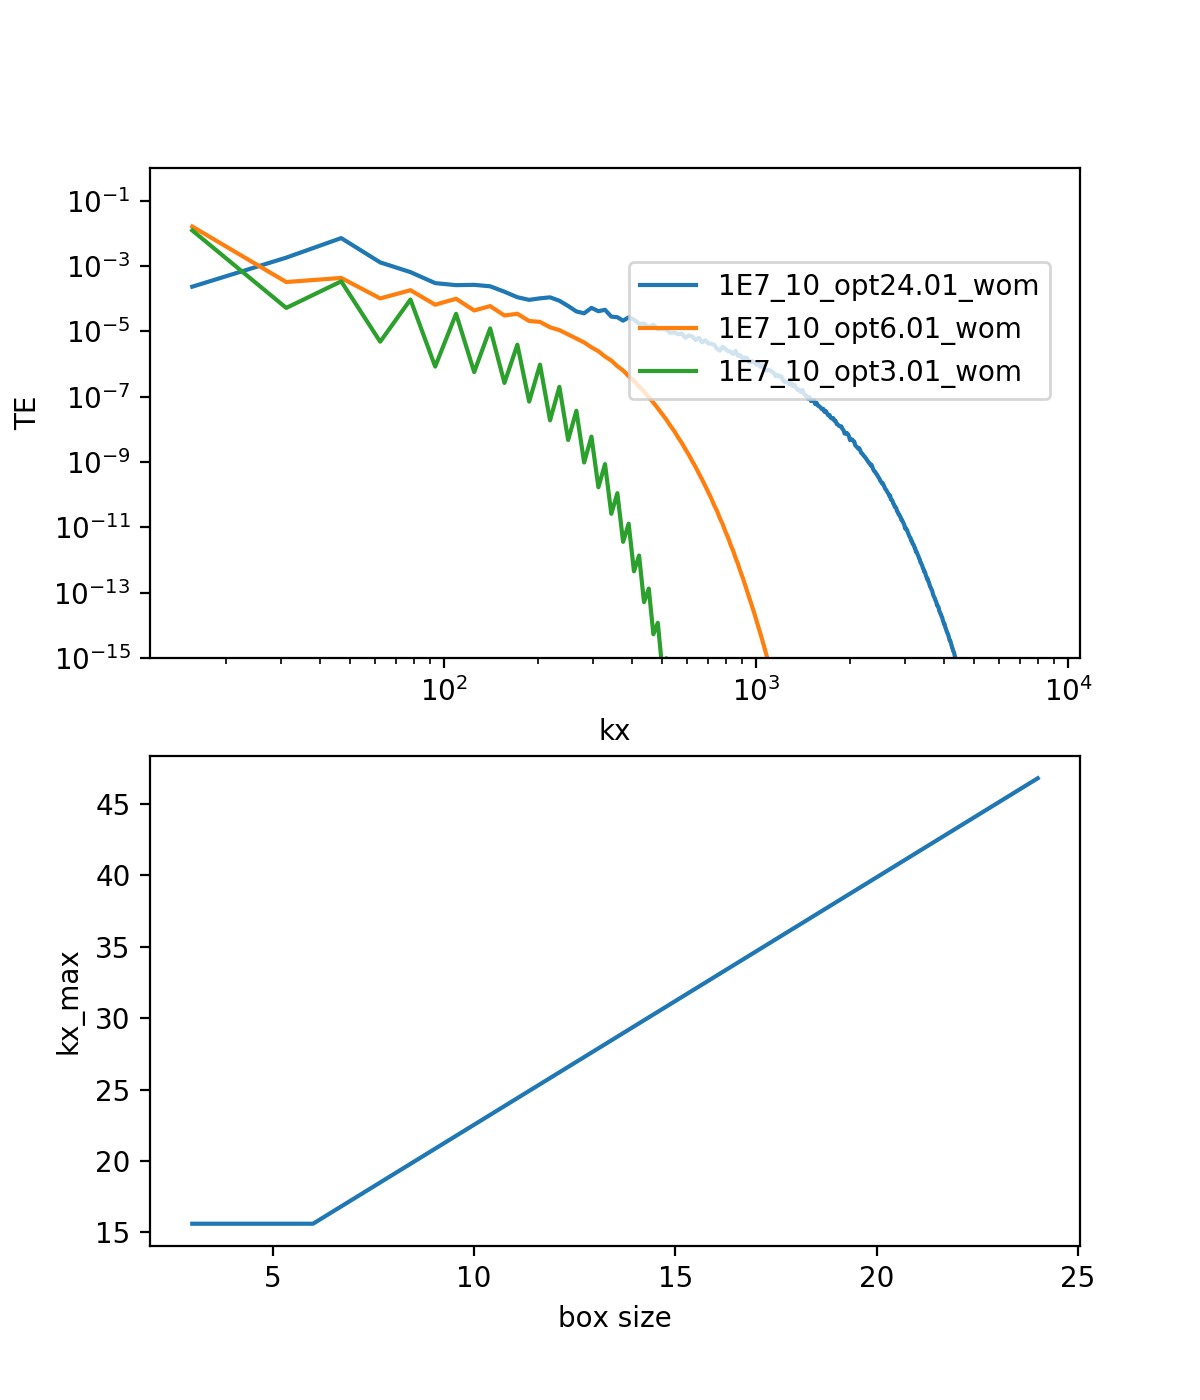
\includegraphics[width=\linewidth]{TE_1E7_10.png}
      	\caption{ Total energy spectra at $Ra = 1E7, Pr =10$ along $y = 0$}
      	\label{fig:fig24}
      \end{figure}
     
     A comparison of the momentum boundary layer for the various cases are shown in Figures 25.  
     
     \begin{figure}[!htb]
     	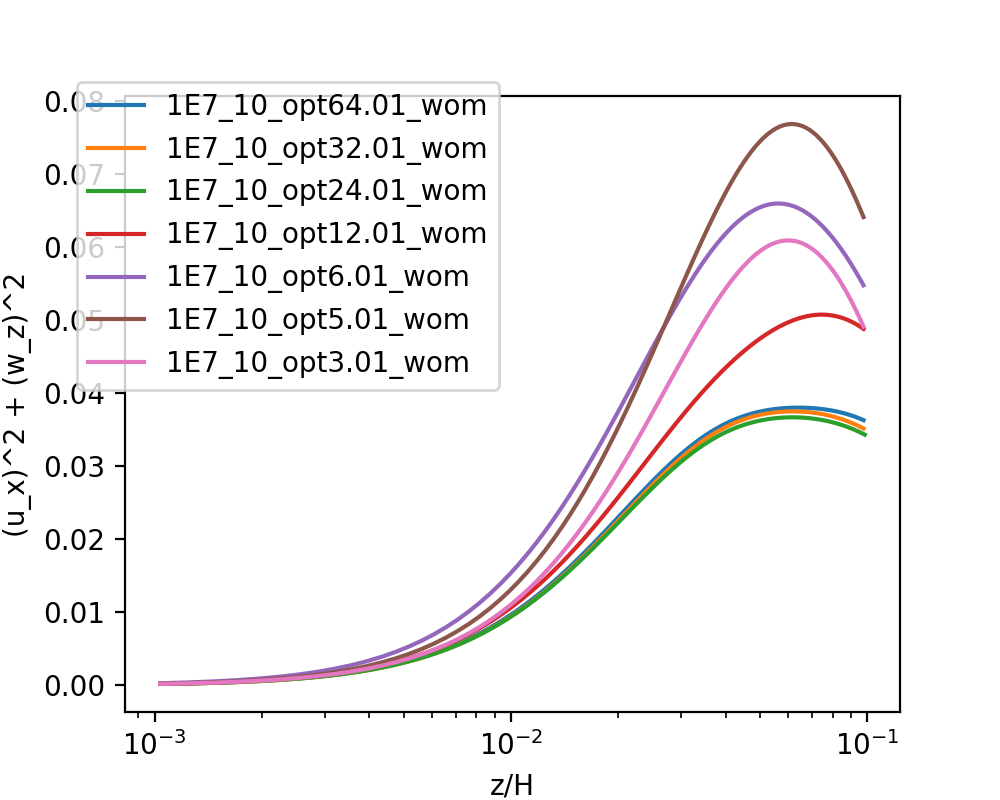
\includegraphics[width=\linewidth]{BL_1E7_10.png}
     	\caption{ Vertical profile of total normal stress magnitude at $Ra = 1E7, Pr =10$ for various box sizes}
     	\label{fig:fig25}
     \end{figure}
    
\end{document}
